\appendix
\begin{center}
  {\Large\bf Appendix to ``Cold-start Playlist Recommendation with Multitask Learning''}
\end{center}
\rule{0pt}{50pt}


%\section{Proof}
\section{Proof of classification objective minimises ranking objective}

The empirical risk $\RCal_\textsc{rank}$ can be approximated (with the exponential surrogate) as follows:
\begin{equation*}
\begin{aligned}
\RCal_\textsc{rank} 
&= \frac{1}{N} \sum_{i=1}^N \frac{1}{M_-^i} \exp \left( -\min_{m: y_m^i = 1} f(i, m) \right) \sum_{n: y_n^i = 0} \exp(f(i, n)) \\
&\approx \frac{1}{N} \sum_{i=1}^N \frac{1}{M_-^i} \exp \left( \frac{1}{p} \log\sum_{m: y_m^i = 1} e^{-p f(i, m)} \right)
         \sum_{n: y_n^i = 0} e^{f(i, n)} \\
&= \frac{1}{N} \sum_{i=1}^N \frac{1}{M_-^i} \exp \left( \log \left( \sum_{m: y_m^i = 1} e^{-p f(i, m)} \right)^\frac{1}{p} \right) 
   \sum_{n: y_n^i = 0} e^{f(i, n)} \\
&= \frac{1}{N} \sum_{i=1}^N \frac{1}{M_-^i} \left( \sum_{m: y_m^i = 1} e^{-p f(i, m)} \right)^\frac{1}{p} \sum_{n: y_n^i = 0} e^{f(i, n)} \\
&= \widetilde\RCal_\textsc{rank}.
\end{aligned}
\end{equation*}

Let $\RCal_\textsc{clf}$ be the following classification risk:
\begin{equation*}
\RCal_\textsc{clf} 
= \frac{1}{N} \sum_{i=1}^N \left( 
  \frac{1}{p M_+^i} \sum_{m: y_m^i = 1} e^{-p f(i, m)} 
  + \frac{1}{M_-^i} \sum_{n: y_n^i = 0} e^{f(i, n)} \right),
\end{equation*}
we have a theorem
\begin{theorem}
Let $\uptheta^* \in \argmin_{\uptheta} \RCal_\textsc{clf}$ (assuming minimisers exist), 
then $\uptheta^* \in \argmin_{\uptheta} \widetilde\RCal_\textsc{rank}$.
\end{theorem}

\begin{proof}
We following the proof technique in~\cite{ertekin2011equivalence}
by first introducing a constant feature $1$ for each song,
without loss of generality, let $x_m^0$ be the constant feature.
Then we can show that
$\frac{\partial \, \RCal_\textsc{clf}} {\partial \, \uptheta} = 0$ implies
$\frac{\partial \, \widetilde\RCal_\textsc{rank}} {\partial \, \uptheta} = 0$,
which means minimisers of $\RCal_\textsc{clf}$ also minimise $\widetilde\RCal_\textsc{rank}$.

First, we introduce a constant feature $1$ for $x_m, \, m \in \{1,\dots,M\}$ to serve as a bias, 
and without loss of generality, let $x_m^0$ be the constant feature, \ie $x_m^0 = 1$, 
$\forall i \in \{1,\dots,N\}$, let
\begin{equation*}
\begin{aligned}
0 
&= \frac{\partial \RCal_\textsc{clf}} {\partial v_i^0}
&= \frac{1}{p M_+^i} \sum_{m: y_m^i = 1} e^{-p f(i, m)} (-p) + \frac{1}{M_-^i} \sum_{n: y_n^i = 0} e^{f(i, n)},
\end{aligned}
\end{equation*}
we have
\begin{equation}
\label{eq:eq1}
\frac{1}{M_+^i} \sum_{m: y_m^i = 1} e^{-p f(i, m)} = \frac{1}{M_-^i} \sum_{n: y_n^i = 0} e^{f(i, n)}.
\end{equation}

Further, let
\begin{equation*}
0 
= \frac{\partial \RCal_\textsc{clf}} {\partial \bv_i} 
= \frac{1}{p M_+^i} \sum_{m: y_m^i = 1} e^{-p f(i, m)} (-p \x_m) + \frac{1}{M_-^i} \sum_{n: y_n^i = 0} e^{f(i, n)} \x_n,
\end{equation*}
we have
\begin{equation}
\label{eq:eq2}
\frac{1}{M_+^i} \sum_{m: y_m^i = 1} e^{-p f(i, m)} \x_m = \frac{1}{M_-^i} \sum_{n: y_n^i = 0} e^{f(i, n)} \x_n.
\end{equation}

Note that
\begin{equation*}
\begin{aligned}
&\frac{\partial \widetilde\RCal_\textsc{rank}} {\partial \bv_i} \\
&= \frac{1}{N M_-^i} \left[ \frac{1}{p} 
   \left( \sum_{m: y_m^i=1} e^{-p f(i, m)} \right)^{\frac{1}{p} - 1} \sum_{m: y_m^i=1} e^{-p f(i, m)} (-p) \x_m \sum_{n: y_n^i=0} e^{f(i, n)}
   + \left( \sum_{m: y_m^i = 1} e^{-p f(i, m)} \right)^\frac{1}{p} \sum_{n: y_n^i = 0} e^{f(i, n)} \x_n \right] \\
&= \frac{-1}{N M_-^i} \left( \sum_{m: y_m^i=1} e^{-p f(i, m)} \right)^{\frac{1}{p} - 1} 
   \left[ \sum_{m: y_m^i=1} e^{-p f(i, m)} \x_m \sum_{n: y_n^i=0} e^{f(i, n)}
   - \sum_{m: y_m^i = 1} e^{-p f(i, m)} \sum_{n: y_n^i = 0} e^{f(i, n)} \x_n \right] \\
&= \frac{-1}{N M_-^i} \left( \sum_{m: y_m^i=1} e^{-p f(i, m)} \right)^{\frac{1}{p} - 1} 
   \left[ \sum_{m: y_m^i=1} e^{-p f(i, m)} \x_m \frac{M_-^i}{M_+^i} \sum_{m: y_m^i=1} e^{-p f(i, m)}
   - \sum_{m: y_m^i = 1} e^{-p f(i, m)} \sum_{n: y_n^i = 0} e^{f(i, n)} \x_n \right] \ \text{(by Eq.~\ref{eq:eq1})} \\
&= \frac{-1}{N M_-^i} \left( \sum_{m: y_m^i=1} e^{-p f(i, m)} \right)^\frac{1}{p} 
   \left[ \frac{M_-^i}{M_+^i} \sum_{m: y_m^i=1} e^{-p f(i, m)} \x_m - \sum_{n: y_n^i = 0} e^{f(i, n)} \x_n \right] \\
&= 0. \ \text{(by Eq.~\ref{eq:eq2})}
\end{aligned}
\end{equation*}

We can similarly prove that 
\begin{equation*}
\begin{aligned}
\frac{\partial \widetilde\RCal_\textsc{rank}}{\partial \bu_j} &= 0, \ \forall j \in \{1,\dots,U\} \\
\frac{\partial \widetilde\RCal_\textsc{rank}}{\partial \widebar{\bu}} &= 0.
\end{aligned}
\end{equation*}

Which means minimisers of $\RCal_\textsc{clf}$ also minimise $\widetilde\RCal_\textsc{rank}$.

\end{proof}





\clearpage
\newpage

\section{Evaluation metrics}
The four evaluation metrics used in this work are:
\begin{itemize}
\item \emph{HitRate@K}, which is also known as Recall@K, is the number of correctly recommended songs amongst the top-$K$ recommendations over
      the number of songs in the observed playlist.
\item \emph{Area under the ROC curve} (AUC), which is the probability that a positive instance is ranked higher than a negative instance (on average).
\item \emph{Novelty} measures the ability of a recommender system to suggest previously unknown (\ie novel) items,
      $$
      \text{Novelty@K} 
      = \frac{1}{U} \sum_{u=1}^U \frac{1}{|P_u^\textsc{test}|} \sum_{i \in P_u^\textsc{test}} \sum_{m \in S_K^i} 
        \frac{-\log_2 pop_m}{K},
      $$
      where $P_u^\textsc{test}$ is the (indices of) test playlists from user $u$, 
      $S_K^i$ is the set of top-$K$ recommendations for test playlist $i$ and $pop_m$ is the popularity of song $m$.
      Intuitively, the more popular a song is, the more likely a user is to be familiar with it, and therefore the less likely to be novel.
\item \emph{Spread} measures the ability of a recommender system to spread its attention across all possible items.
      It is defined as the entropy of the distribution of all songs,
      $$
      \text{Spread} = -\sum_{m=1}^M P(m) \log P(m),
      $$
      where $P(m)$ denotes the probability of song $m$ being recommended,
      which is computed from the scores of all possible songs using the \emph{softmax} function in this work.
\end{itemize}


\clearpage
\newpage
\twocolumn

% span two columns
\twocolumn[
\section{Dataset}
\rule{0pt}{10pt}  % gap
]

%\begin{figure*}[!t]
    \centering
    \begin{minipage}{.5\textwidth}
        \centering
        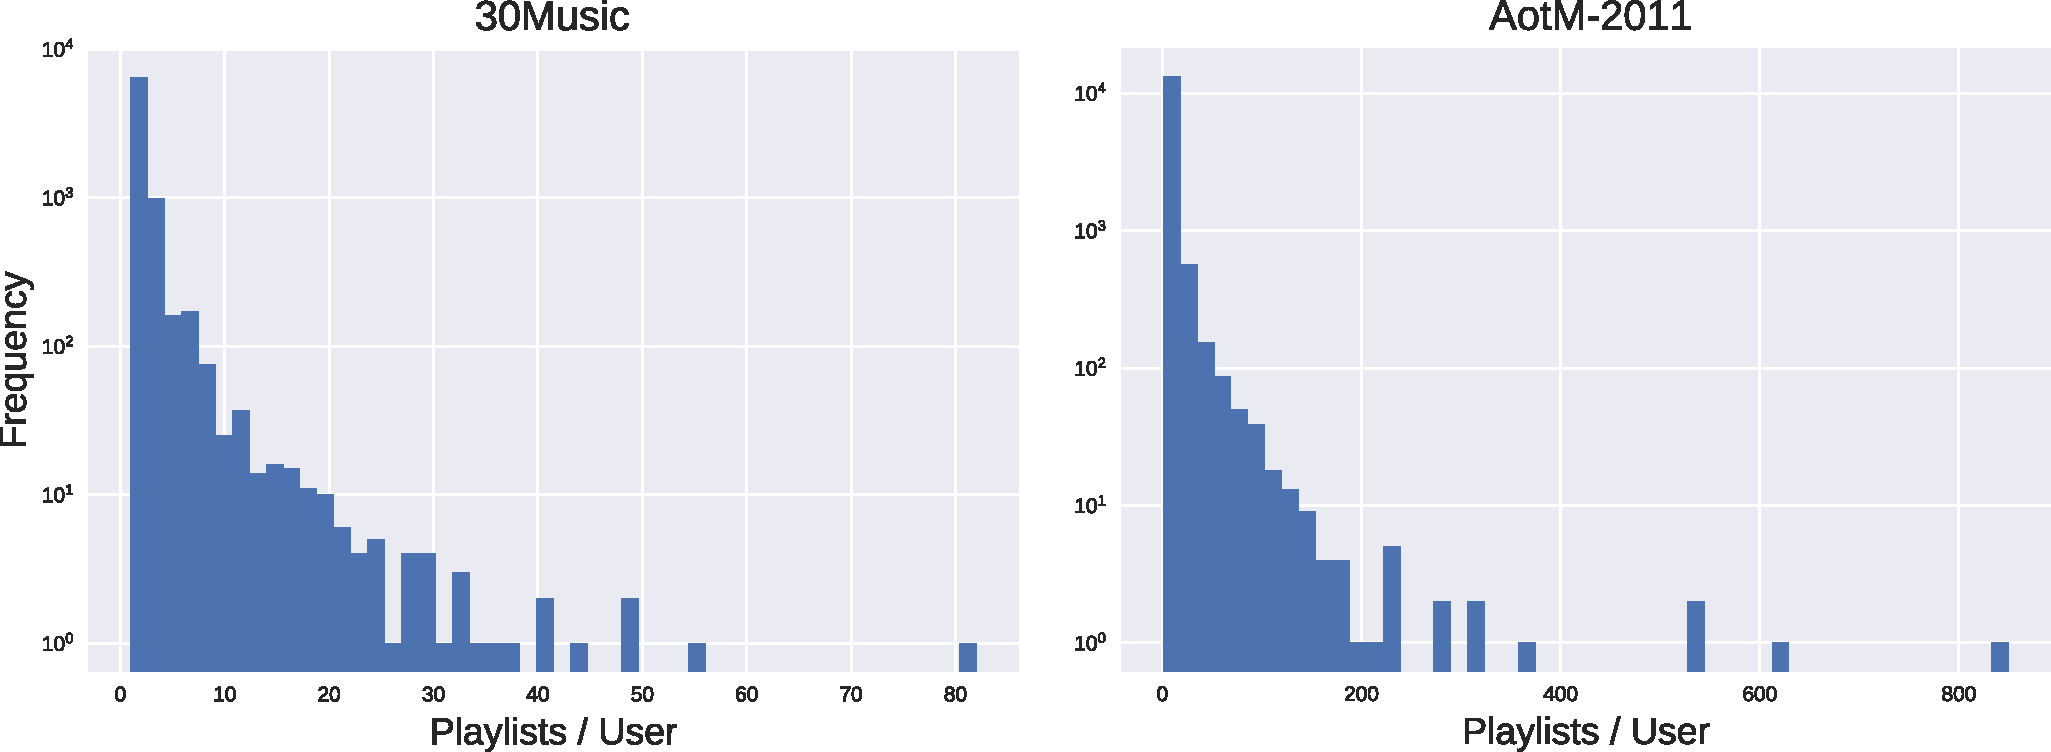
\includegraphics[width=.98\linewidth]{fig/hist_pluser.pdf}
        \caption{Histogram of the number of playlists per user}
        \label{fig:hist_pluser}
    \end{minipage}%
    \begin{minipage}{0.5\textwidth}
        \centering
        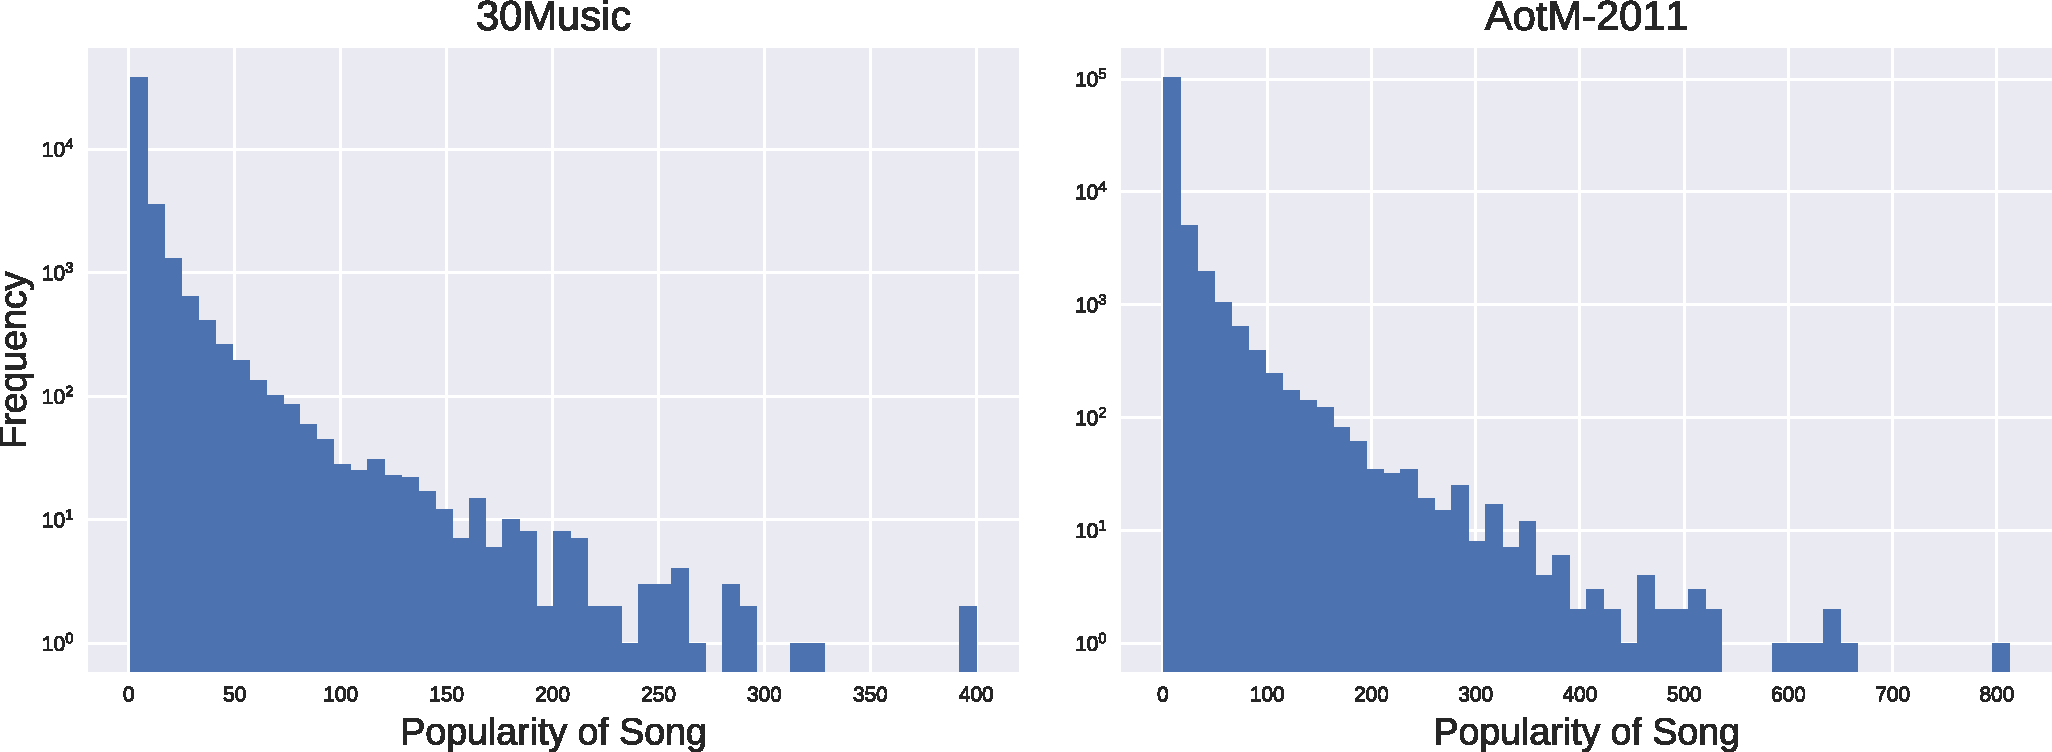
\includegraphics[width=.98\linewidth]{fig/hist_songpop.pdf}
        \caption{Histogram of song popularity}
        \label{fig:hist_songpop}
    \end{minipage}
\end{figure*}

The histograms of the number of playlists per user as well as song popularity 
(\ie the number of occurrences of a song in all playlists)
of the two datasets are shown in Figure~\ref{fig:hist_pluser} and Figure~\ref{fig:hist_songpop},
respectively.
We can see from Figure~\ref{fig:hist_pluser} and \ref{fig:hist_songpop} that both the number
of playlists per user and song popularity follow a long-tailed distribution, which imposes further challenge to the learning task 
as the amount of data is very limited for users (or songs) at the tail.


\begin{figure}[!h]
    \centering
    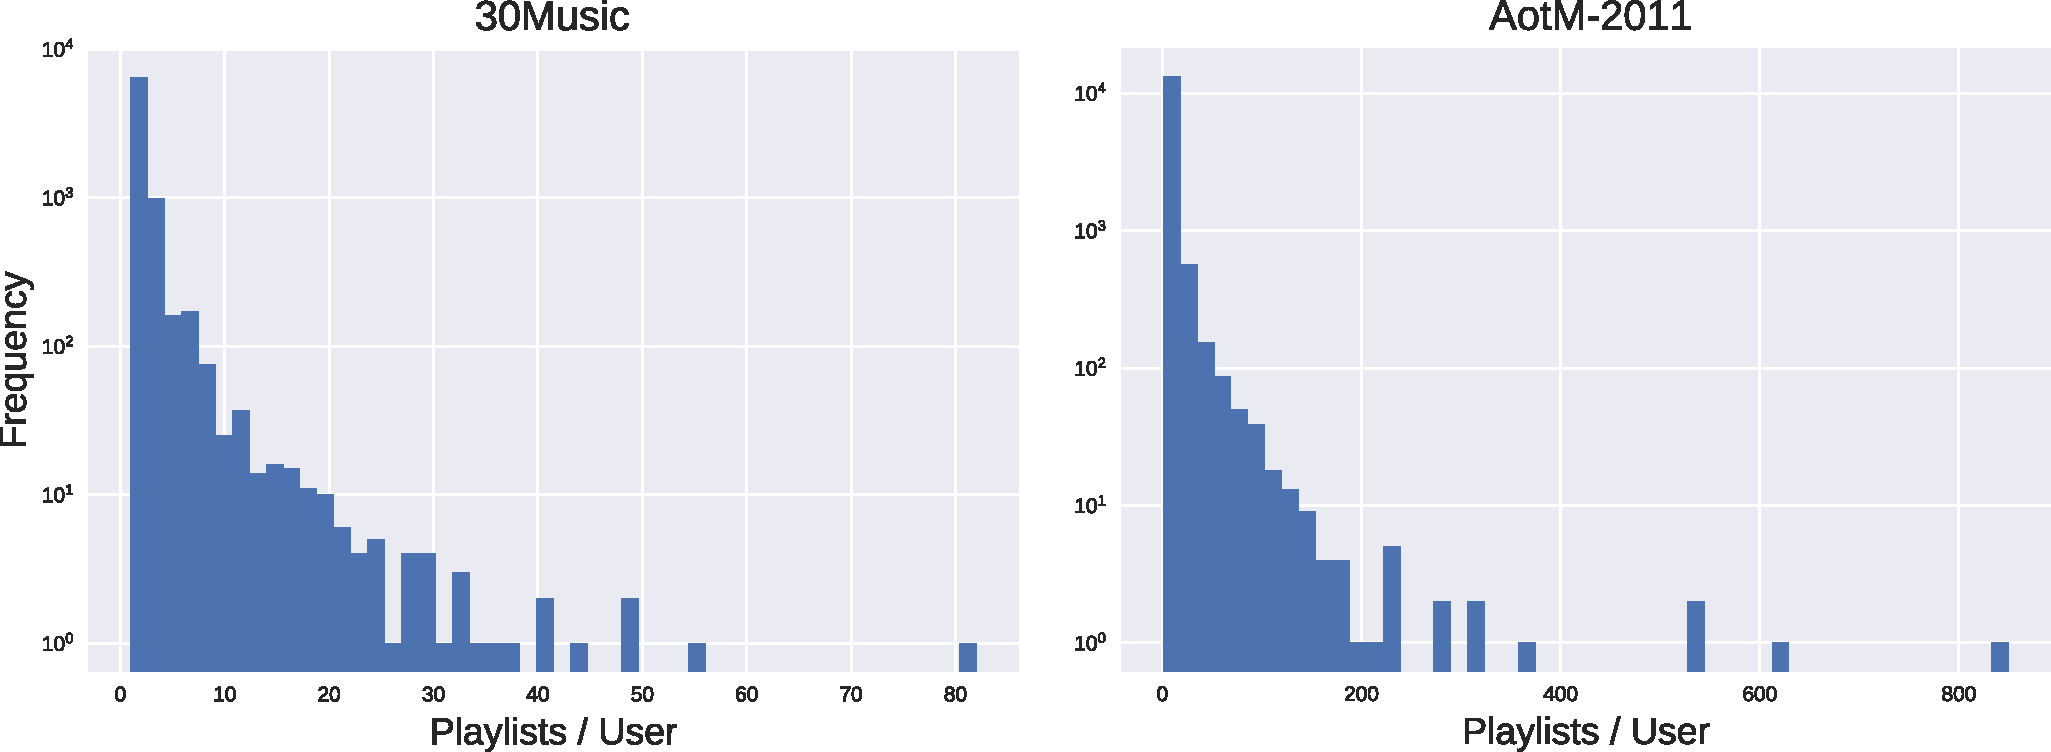
\includegraphics[width=.98\columnwidth]{fig/hist_pluser.pdf}
    \caption{Histogram of the number of playlists per user}
    \label{fig:hist_pluser}
\end{figure}

\begin{figure}[!h]
    \centering
    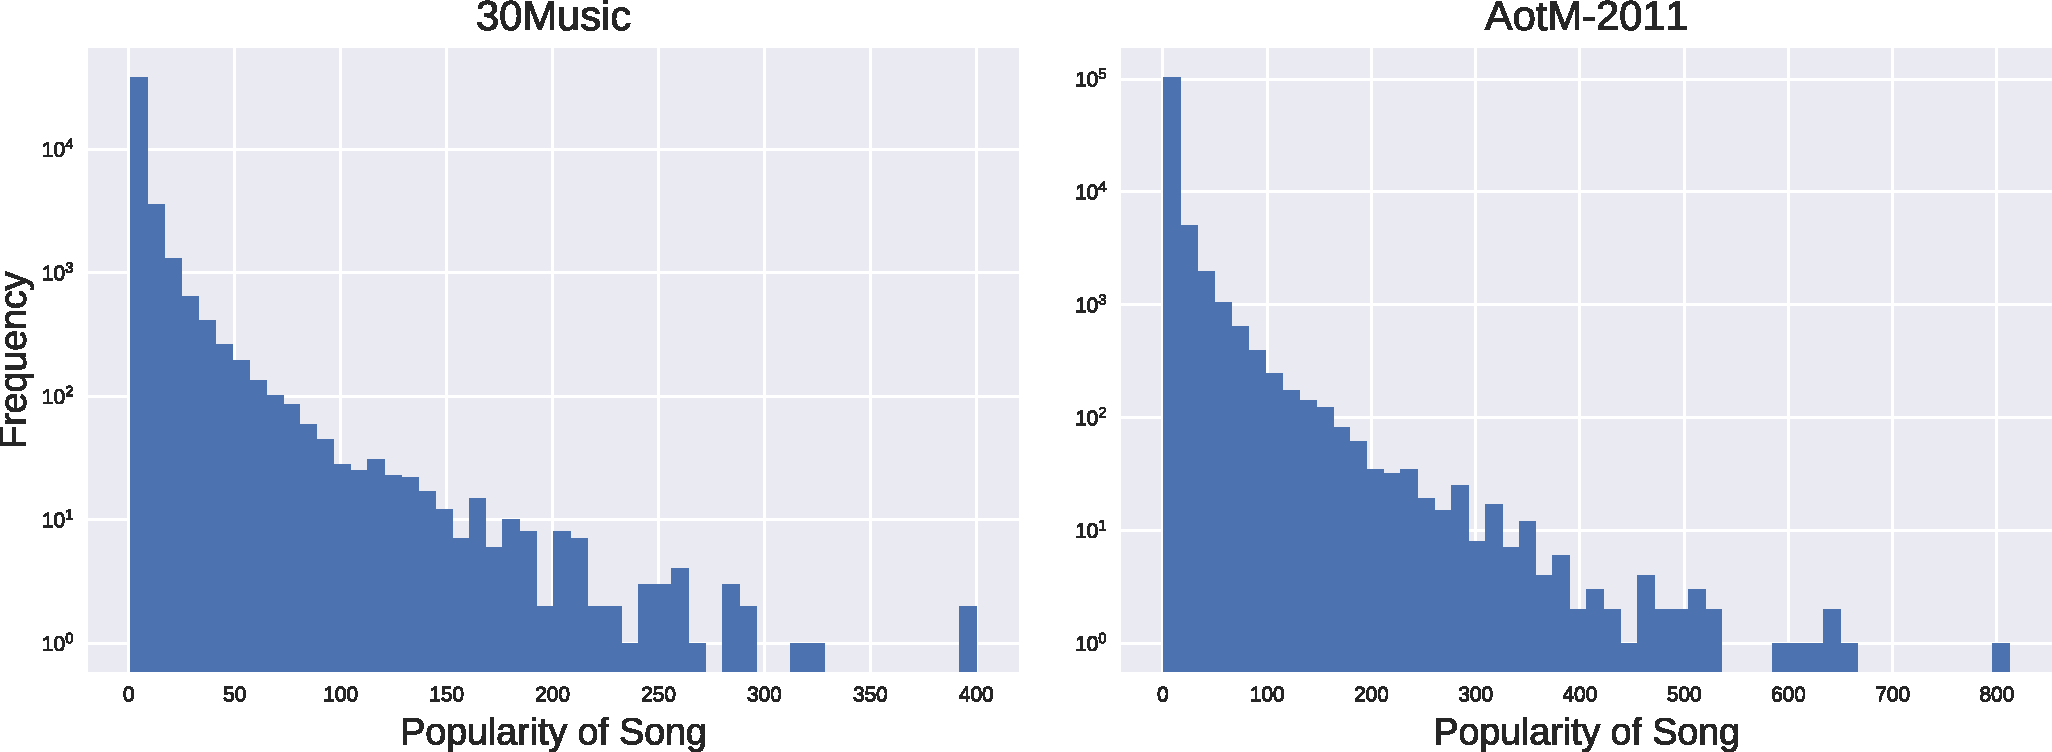
\includegraphics[width=.98\columnwidth]{fig/hist_songpop.pdf}
    \caption{Histogram of song popularity}
    \label{fig:hist_songpop}
\end{figure}

The histograms of the number of playlists per user as well as song popularity 
%(\ie the number of occurrences of a song in all playlists)
of the two datasets are shown in Figure~\ref{fig:hist_pluser} and Figure~\ref{fig:hist_songpop},
respectively.
We can see from Figure~\ref{fig:hist_pluser} and Figure~\ref{fig:hist_songpop} that both the number
of playlists per user and song popularity follow a long-tailed distribution, which imposes further challenge to the learning task 
as the amount of data is very limited for users (or songs) at the tail.

\newpage

The training and test split of the two playlist datasets in the three cold-start settings are shown in 
Table~\ref{tab:stats3}, Table~\ref{tab:stats4}, and Table~\ref{tab:stats1}, respectively.
%\begin{table*}[!t]
    \centering
    \begin{minipage}{.35\textwidth}
        \centering
        \caption{Dataset for \emph{cold songs}}
        \label{tab:stats0}
        \resizebox{.9\textwidth}{!}{
        \begin{tabular}{lrrcrr}
        \toprule
        \multirow{2}{*}{Dataset}  & \multicolumn{2}{c}{Songs} && \multicolumn{2}{c}{Playlists} \\ \cmidrule{2-3} \cmidrule{5-6}
                                  & Train & Test && Train & Test \\
        \midrule
        30Music   & 40,468  & 5,000  && 17,342  & 8,215 \\
        AotM-2011 & 104,428 & 10,000 && 84,646  & 19,504 \\
        \bottomrule
        \end{tabular}
        }
    \end{minipage}%
    \begin{minipage}{0.33\textwidth}
        \centering
        \caption{Dataset for \emph{cold playlists}}
        \label{tab:stats1}
        \resizebox{.9\textwidth}{!}{
        \begin{tabular}{lrrcrr}
        \toprule
        \multirow{2}{*}{Dataset}  & \multicolumn{2}{c}{Playlists} && \multicolumn{2}{c}{Users} \\ \cmidrule{2-3} \cmidrule{5-6}
                                  & Train & Test && Train & Test \\
        \midrule
        30Music   & 15,262 & 2,195 &&  8,070 & 1,644 \\
        AotM-2011 & 75,477 & 9,233 && 14,182 & 2,722 \\
        \bottomrule
        \end{tabular}
        }
    \end{minipage}%
    \begin{minipage}{.33\textwidth}
        \centering
        \caption{Dataset for \emph{cold users}}
        \label{tab:stats2}
        \resizebox{.9\textwidth}{!}{
        \begin{tabular}{lrrcrr}
        \toprule
        \multirow{2}{*}{Dataset}  & \multicolumn{2}{c}{Playlists} && \multicolumn{2}{c}{Users} \\ \cmidrule{2-3} \cmidrule{5-6}
                                  & Train & Test && Train & Test \\
        \midrule
        30Music   & 14,067 & 3,390 && 5,649 & 2,421 \\
        AotM-2011 & 76,450 & 8,260 && 9,928 & 4,254 \\
        \bottomrule
        \end{tabular}
        }
    \end{minipage}
\end{table*}


\begin{table}[!h]
    \centering
    %\setlength\tabcolsep{3pt}
    \caption{Dataset for \emph{cold playlists}}
    \label{tab:stats3}
    \begin{tabular}{lrrcrr}
        \toprule
        \multirow{2}{*}{Dataset}  & \multicolumn{2}{c}{Training Set} && \multicolumn{2}{c}{Test Set} \\ \cmidrule{2-3} \cmidrule{5-6}
                                  & Playlists & Users && Playlists & Users \\
        \midrule
        30Music   & 15,262 &  8,070 && 2,195  & 1,644 \\
        AotM-2011 & 75,477 & 14,182 && 9,233  & 2,722 \\
        \bottomrule
    \end{tabular}
\end{table}

\begin{table}[!h]
    \centering
    \caption{Dataset for \emph{cold users}}
    \label{tab:stats4}
    \begin{tabular}{lrrcrr}
        \toprule
        \multirow{2}{*}{Dataset}  & \multicolumn{2}{c}{Training Set} && \multicolumn{2}{c}{Test Set} \\ \cmidrule{2-3} \cmidrule{5-6}
                                  & Users & Playlists && Users & Playlists \\
        \midrule
        30Music   & 5,649 & 14,067 && 2,420 & 3,390 \\
        AotM-2011 & 9,928 & 76,450 && 4,254 & 8,260 \\
        \bottomrule
    \end{tabular}
\end{table}

\begin{table}[!h]
    \centering
    \caption{Dataset for \emph{cold songs}}
    \label{tab:stats1}
    \begin{tabular}{lrrcrr}
        \toprule
        \multirow{2}{*}{Dataset}  & \multicolumn{2}{c}{Training Set} && \multicolumn{2}{c}{Test Set} \\ \cmidrule{2-3} \cmidrule{5-6}
                                  & Songs & Playlists && Songs & Playlists \\
        \midrule
        30Music   & 40,468  & 17,342 && 5,000  & 8,215 \\
        AotM-2011 & 104,428 & 84,646 && 10,000 & 19,504 \\
        \bottomrule
    \end{tabular}
\end{table}


\clearpage
\newpage
\onecolumn

% span two columns
%\twocolumn[
\section{Empirical results}
%\rule{0pt}{10pt}  % gap
%]

%\begin{figure*}[!t]
    \centering
    \begin{minipage}{0.32\textwidth}
        \centering
        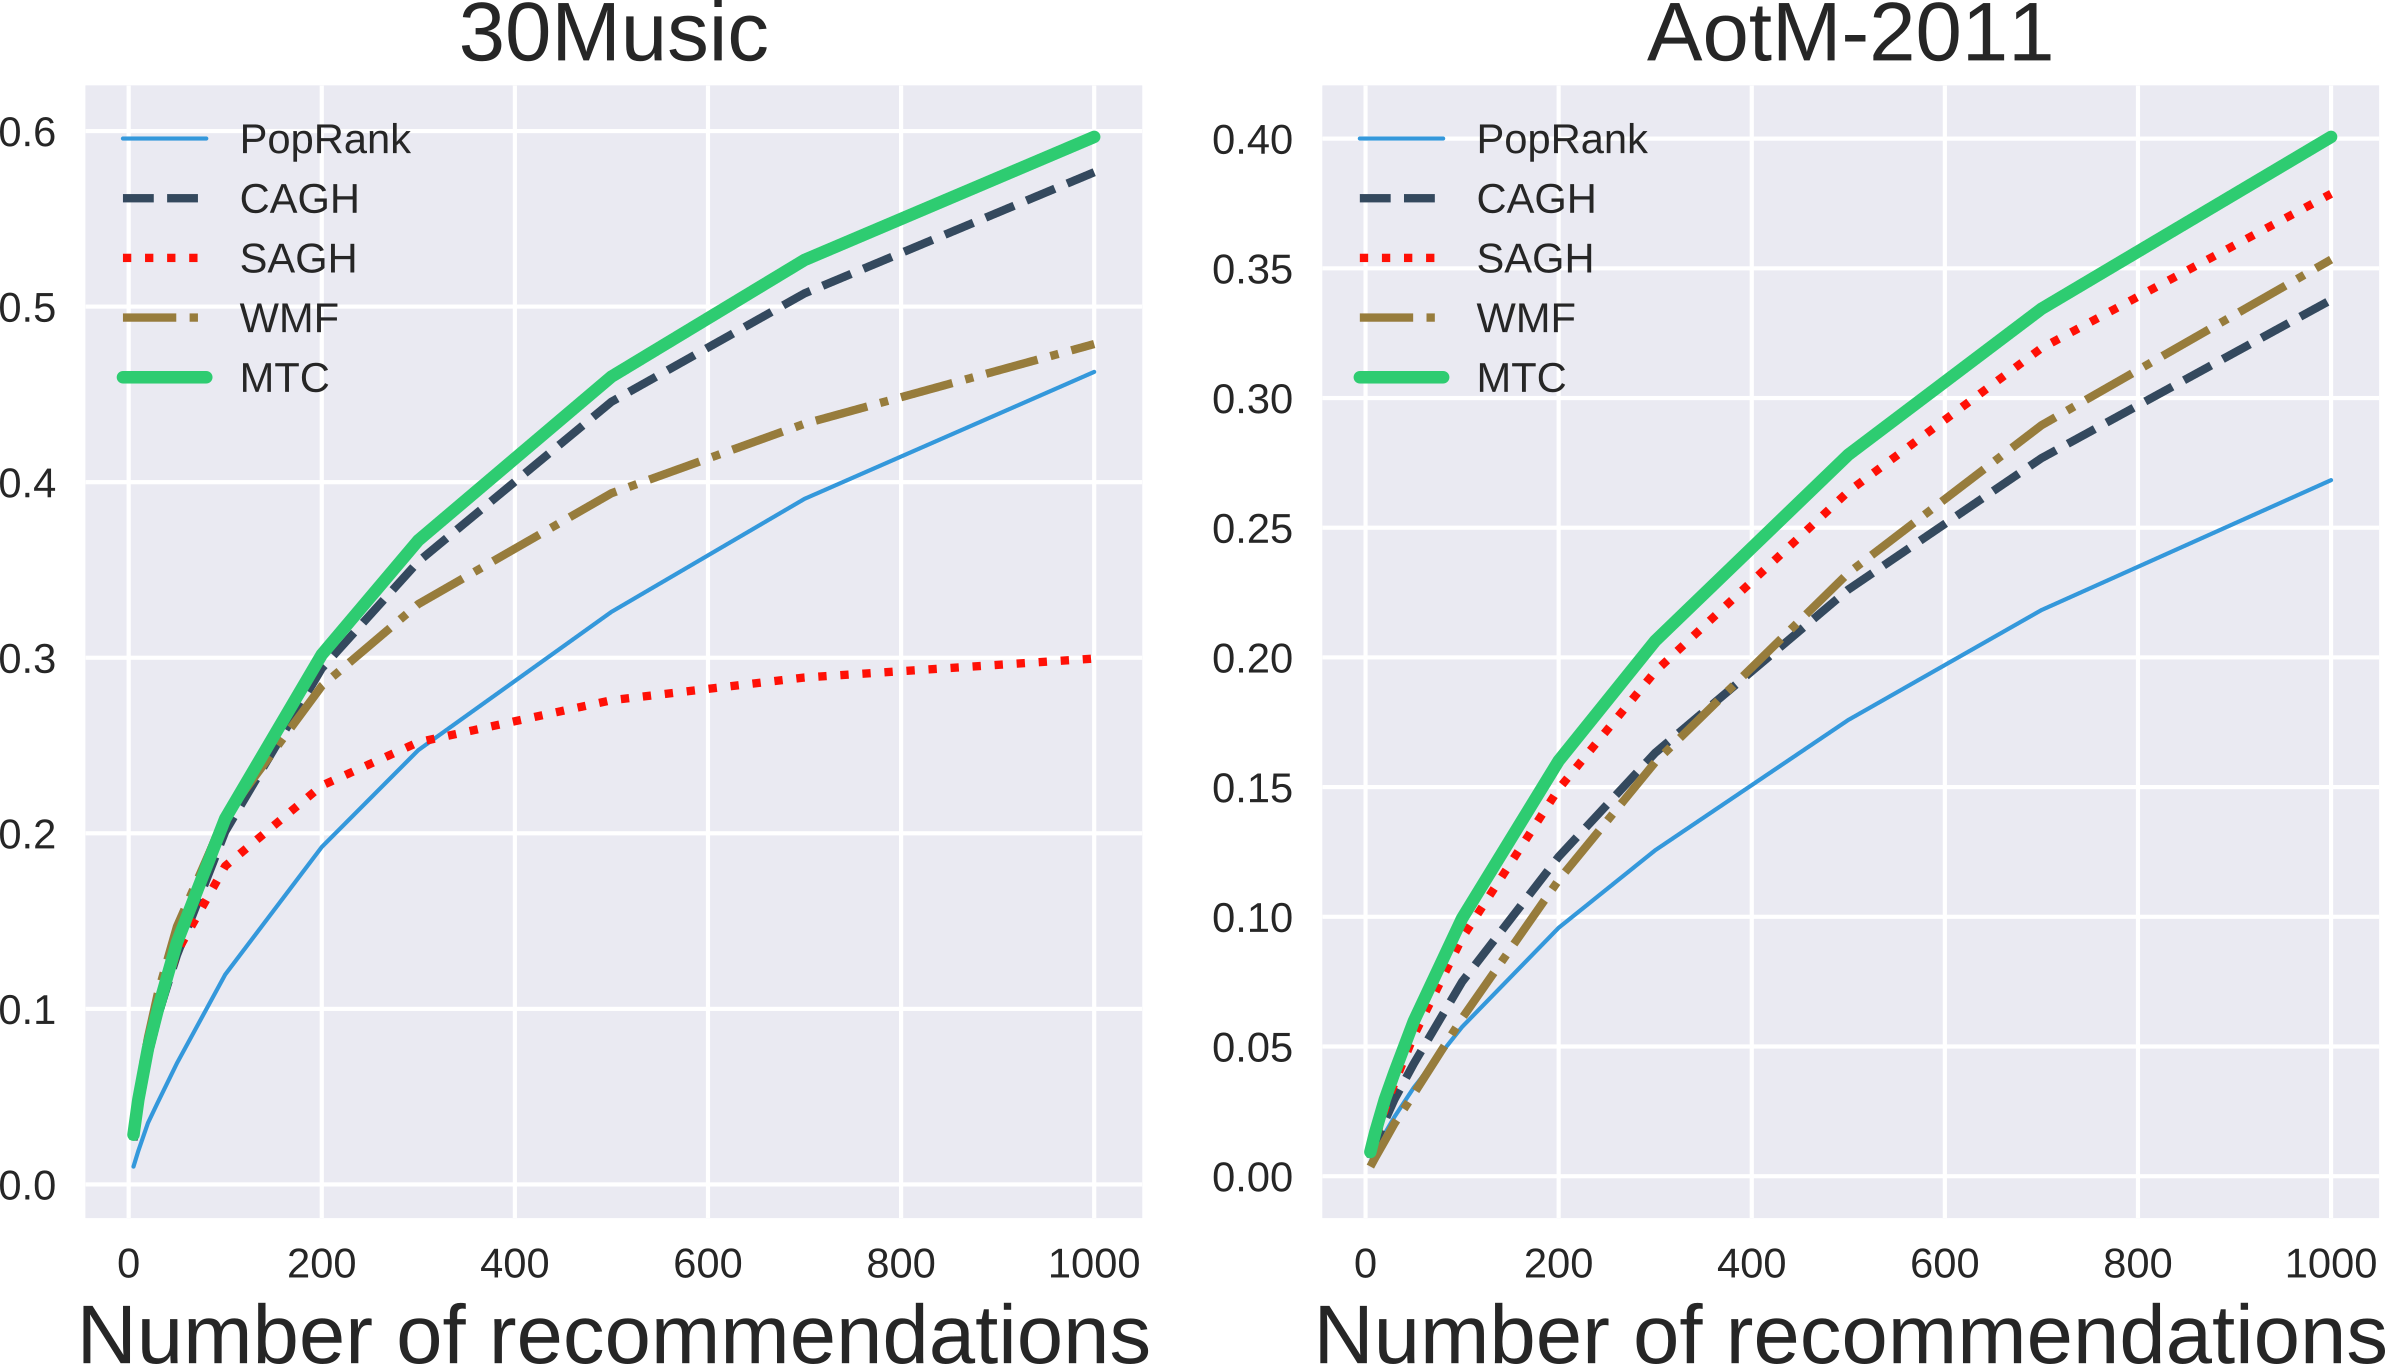
\includegraphics[width=.96\linewidth]{fig/hr3.png}
        \caption{Hit rates for {\it cold playlists}}
        \label{fig:hr3}
    \end{minipage}\hspace{8pt}%
    \begin{minipage}{.32\textwidth}
        \centering
        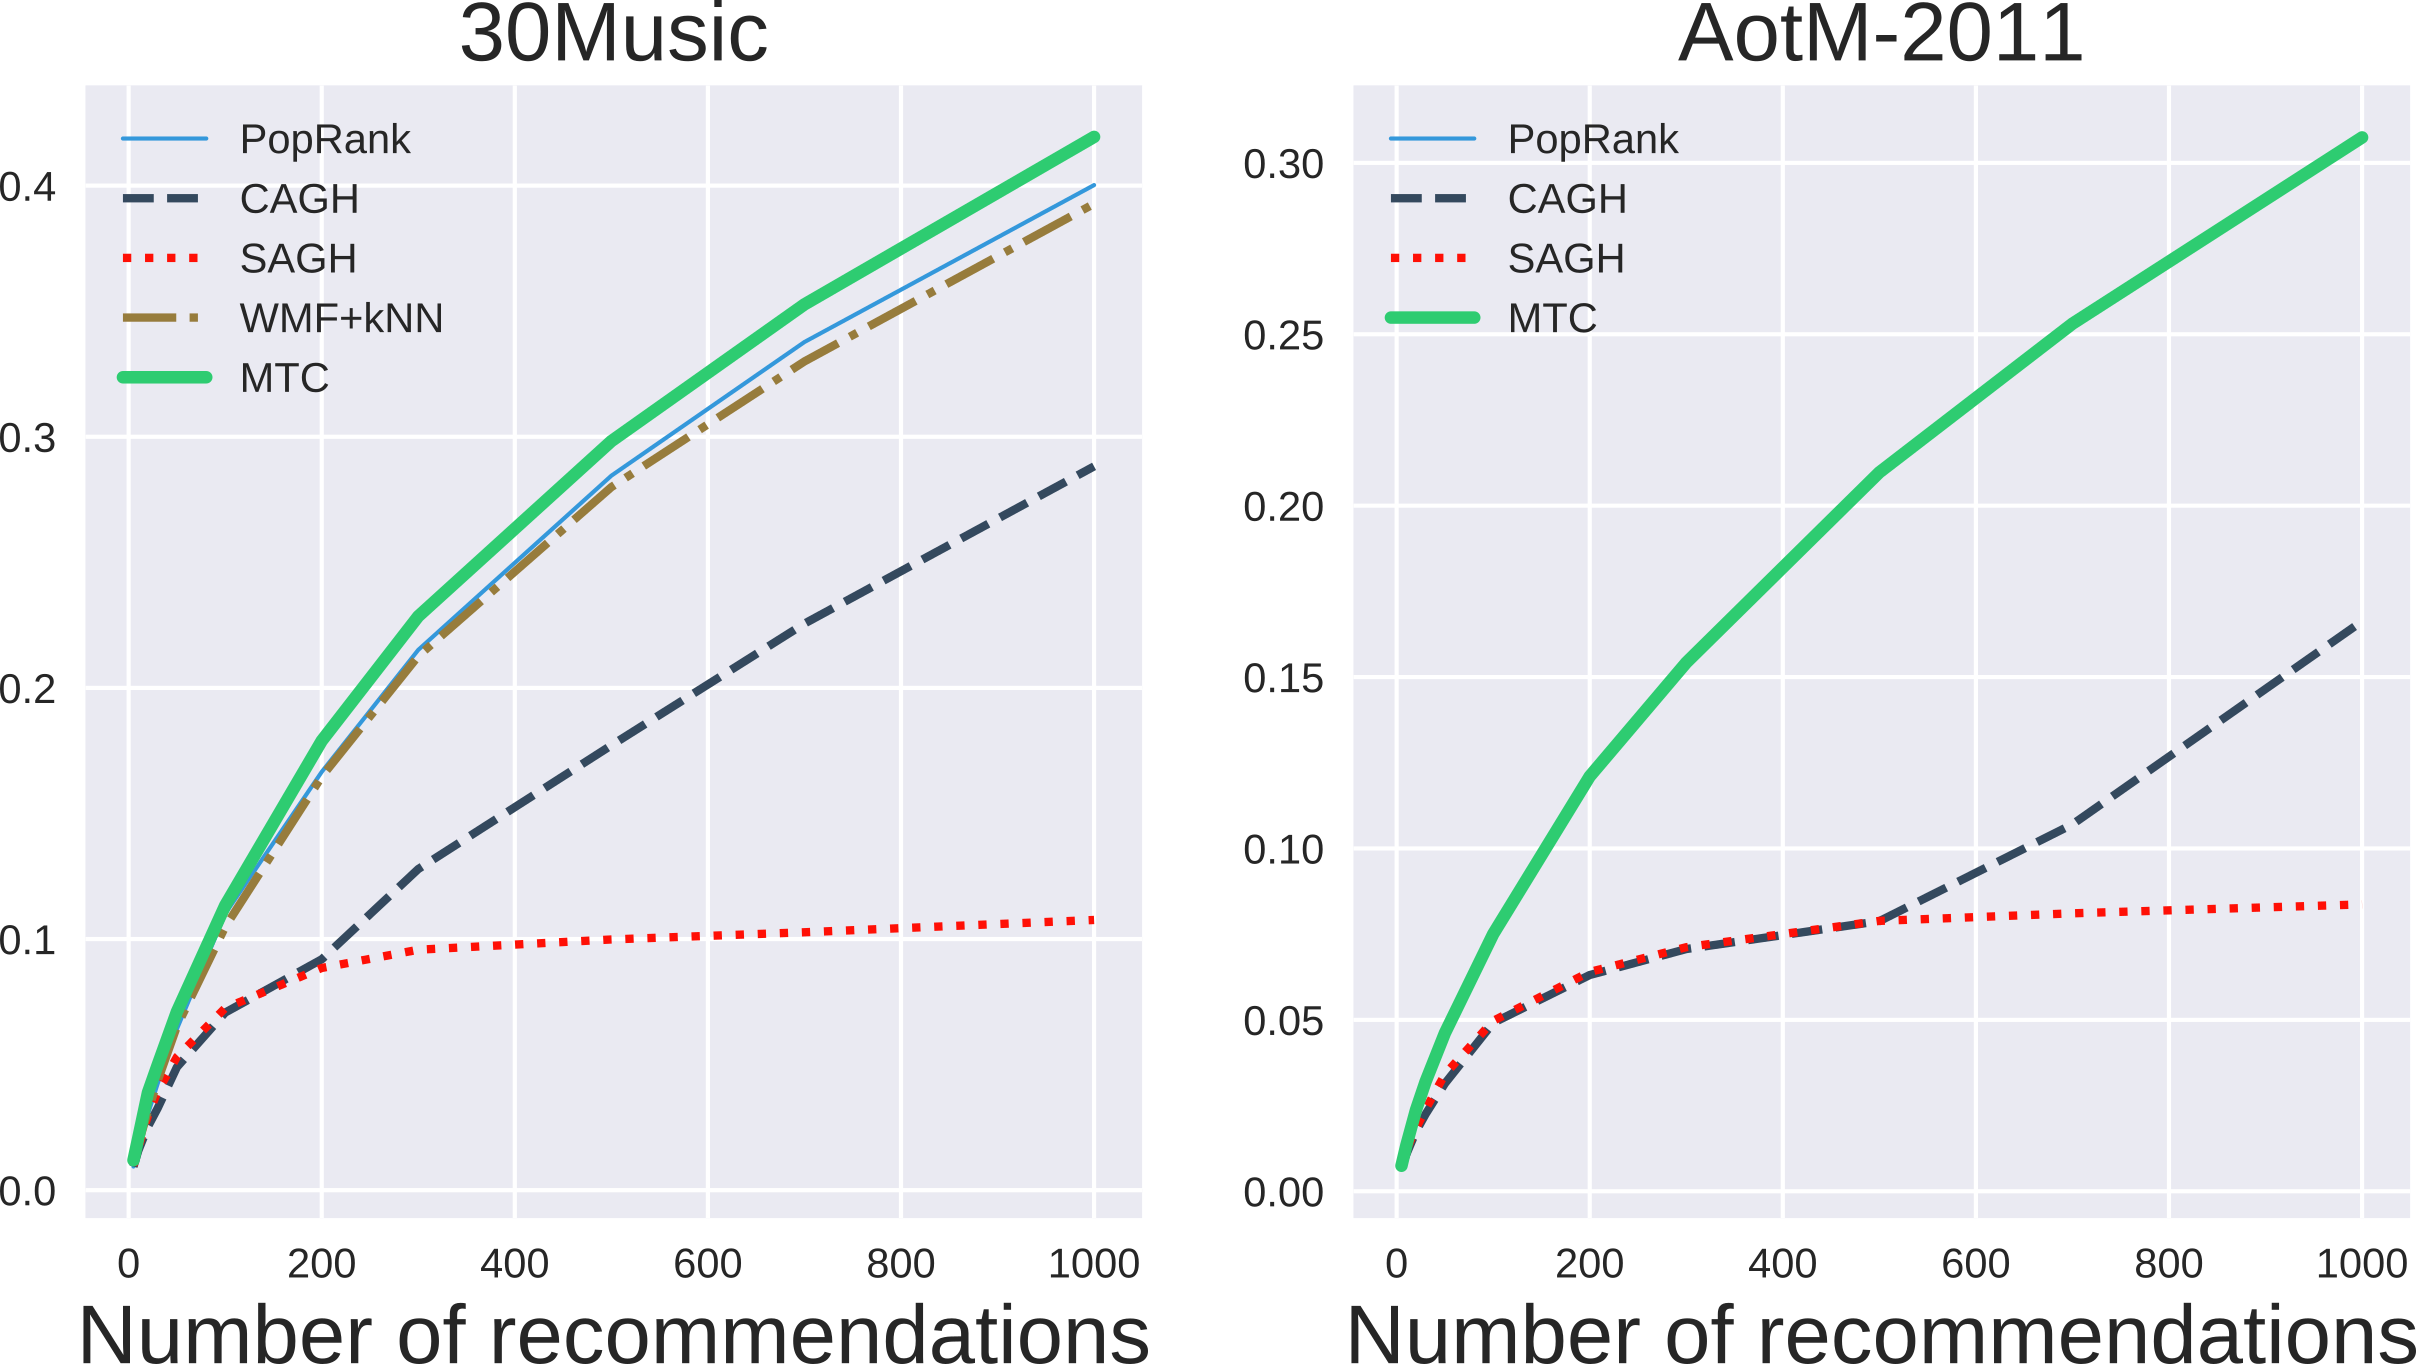
\includegraphics[width=.96\linewidth]{fig/hr4.png}
        \caption{Hit rates for {\it cold users}}
        \label{fig:hr4}
    \end{minipage}\hspace{11pt}%
    \begin{minipage}{0.32\textwidth}
        \centering
        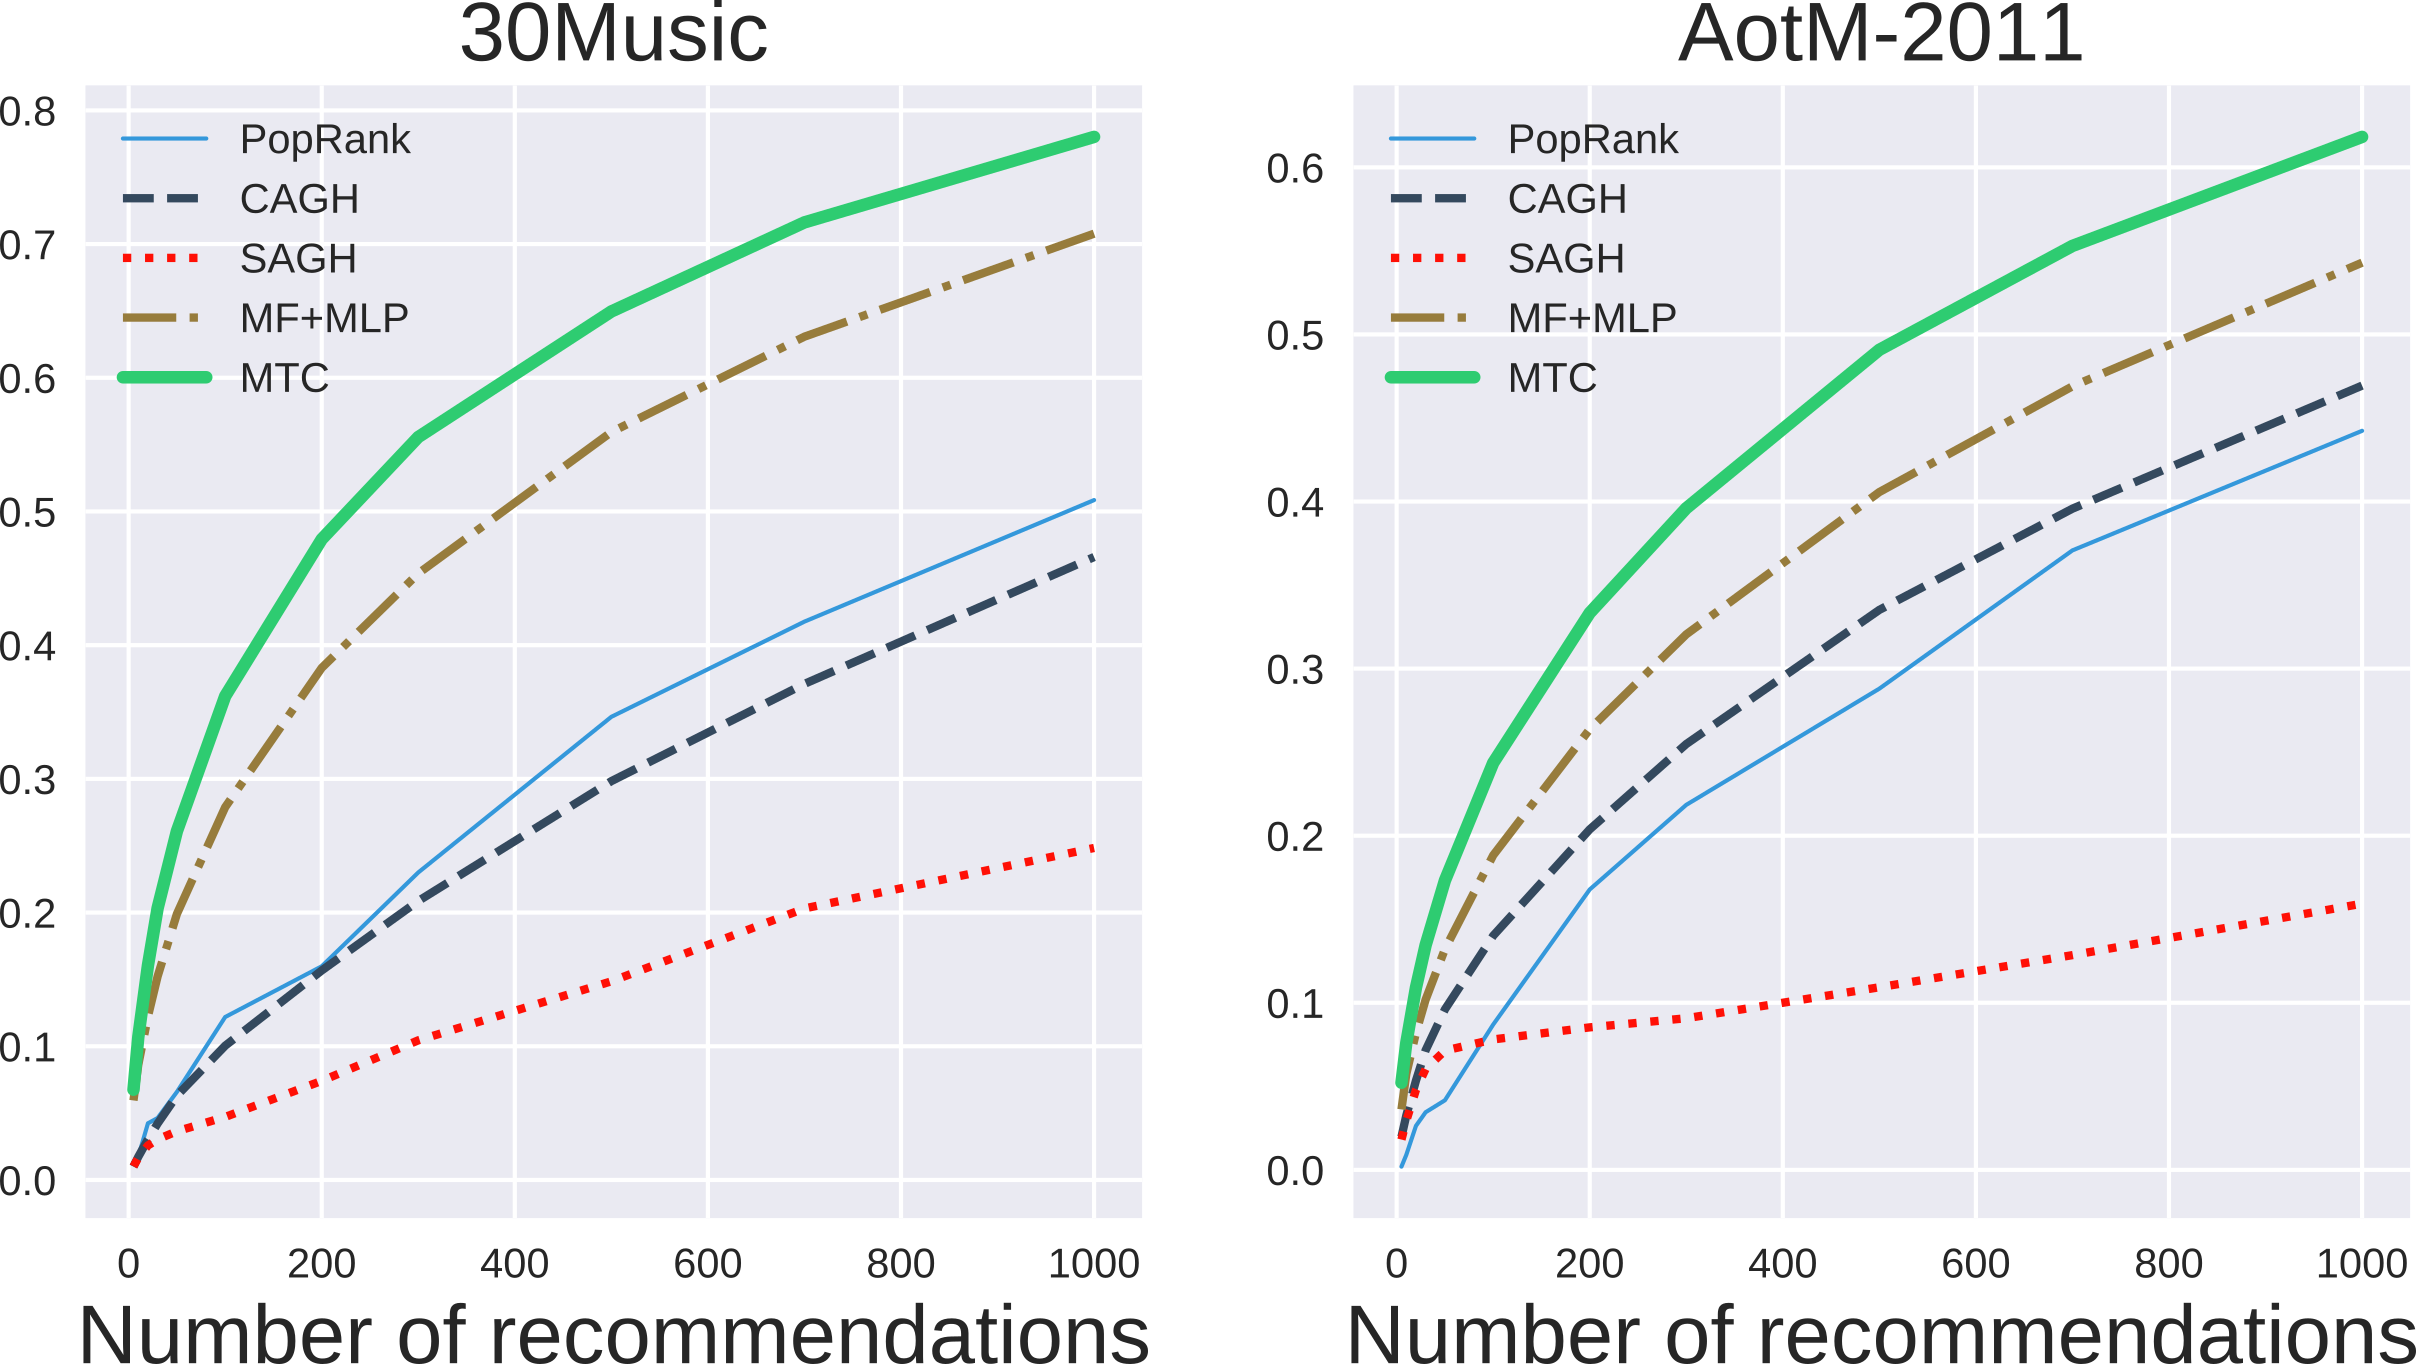
\includegraphics[width=\linewidth]{fig/hr1.png}
        \caption{Hit rates for {\it cold songs}}
        \label{fig:hr1}
    \end{minipage}
\end{figure*}

%\begin{figure*}[!t]
    \begin{minipage}{.5\textwidth}
        \centering
        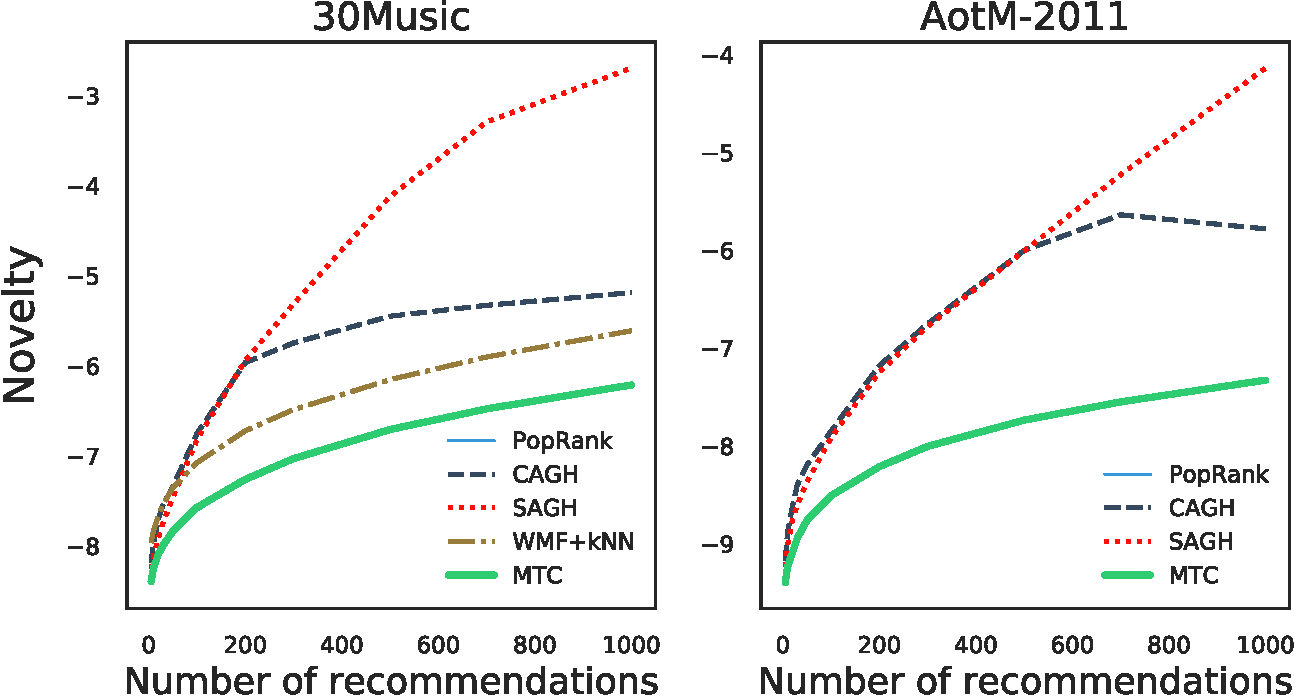
\includegraphics[width=.95\linewidth]{fig/nov4.pdf}
        \caption{Novelty for {\it cold users}}
        \label{fig:hr4}
    \end{minipage}%
    \begin{minipage}{0.5\textwidth}
        \centering
        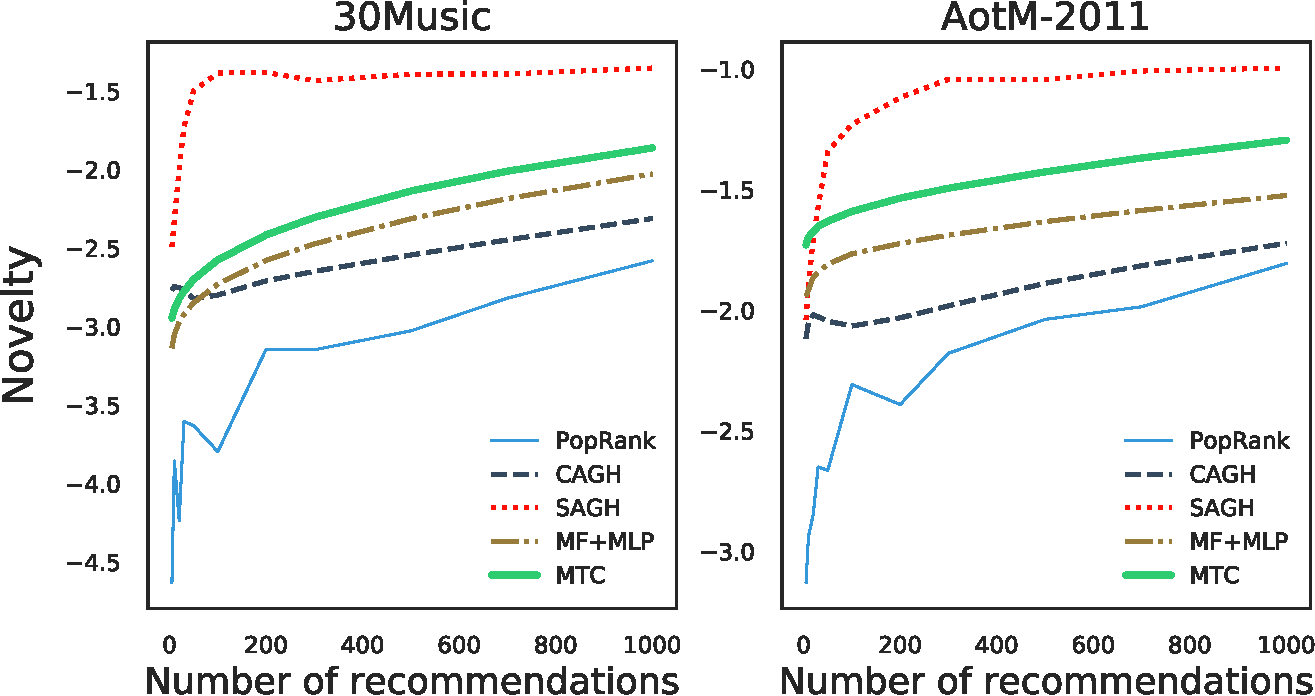
\includegraphics[width=.95\linewidth]{fig/nov1.pdf}
        \caption{Novelty for {\it cold songs}}
        \label{fig:hr1}
    \end{minipage}
\end{figure*}

%\begin{figure}[!t]
    \centering
    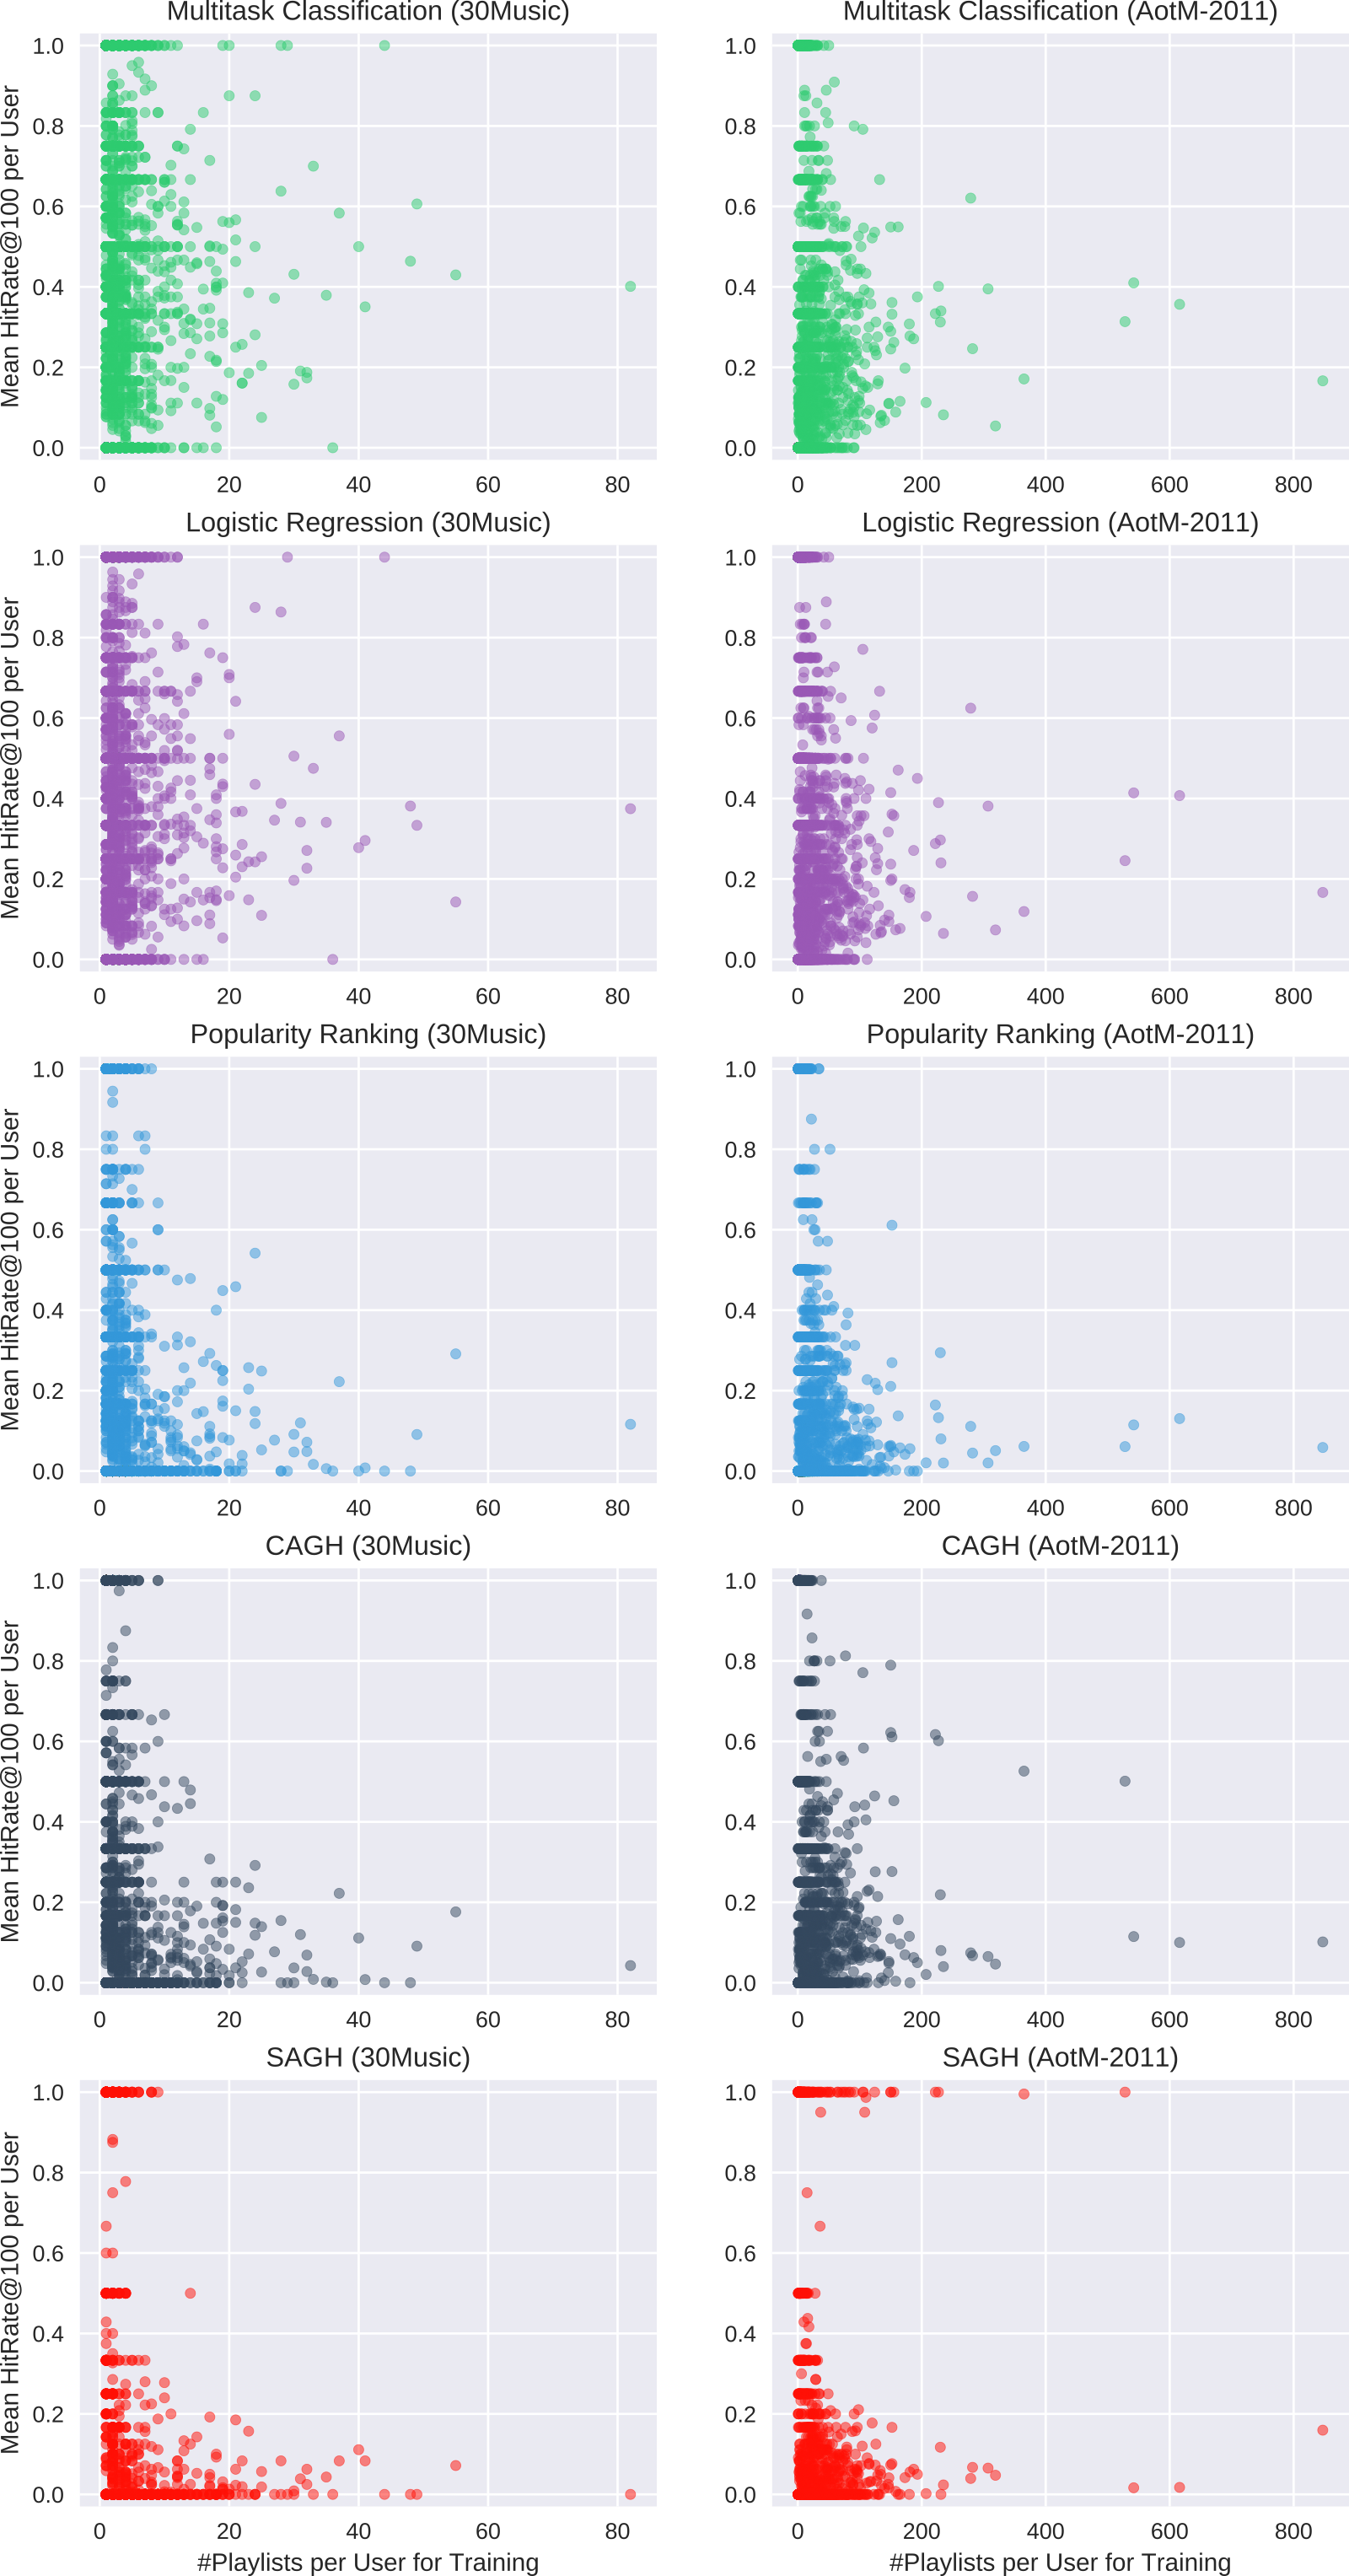
\includegraphics[height=\textheight]{fig/hitrate_per_user0.png}
    \caption{Performance (HitRate@100) per User in \emph{Cold Songs} Setting}
    %\caption{}
    %\label{}
\end{figure}

\begin{figure}[!t]
    \centering
    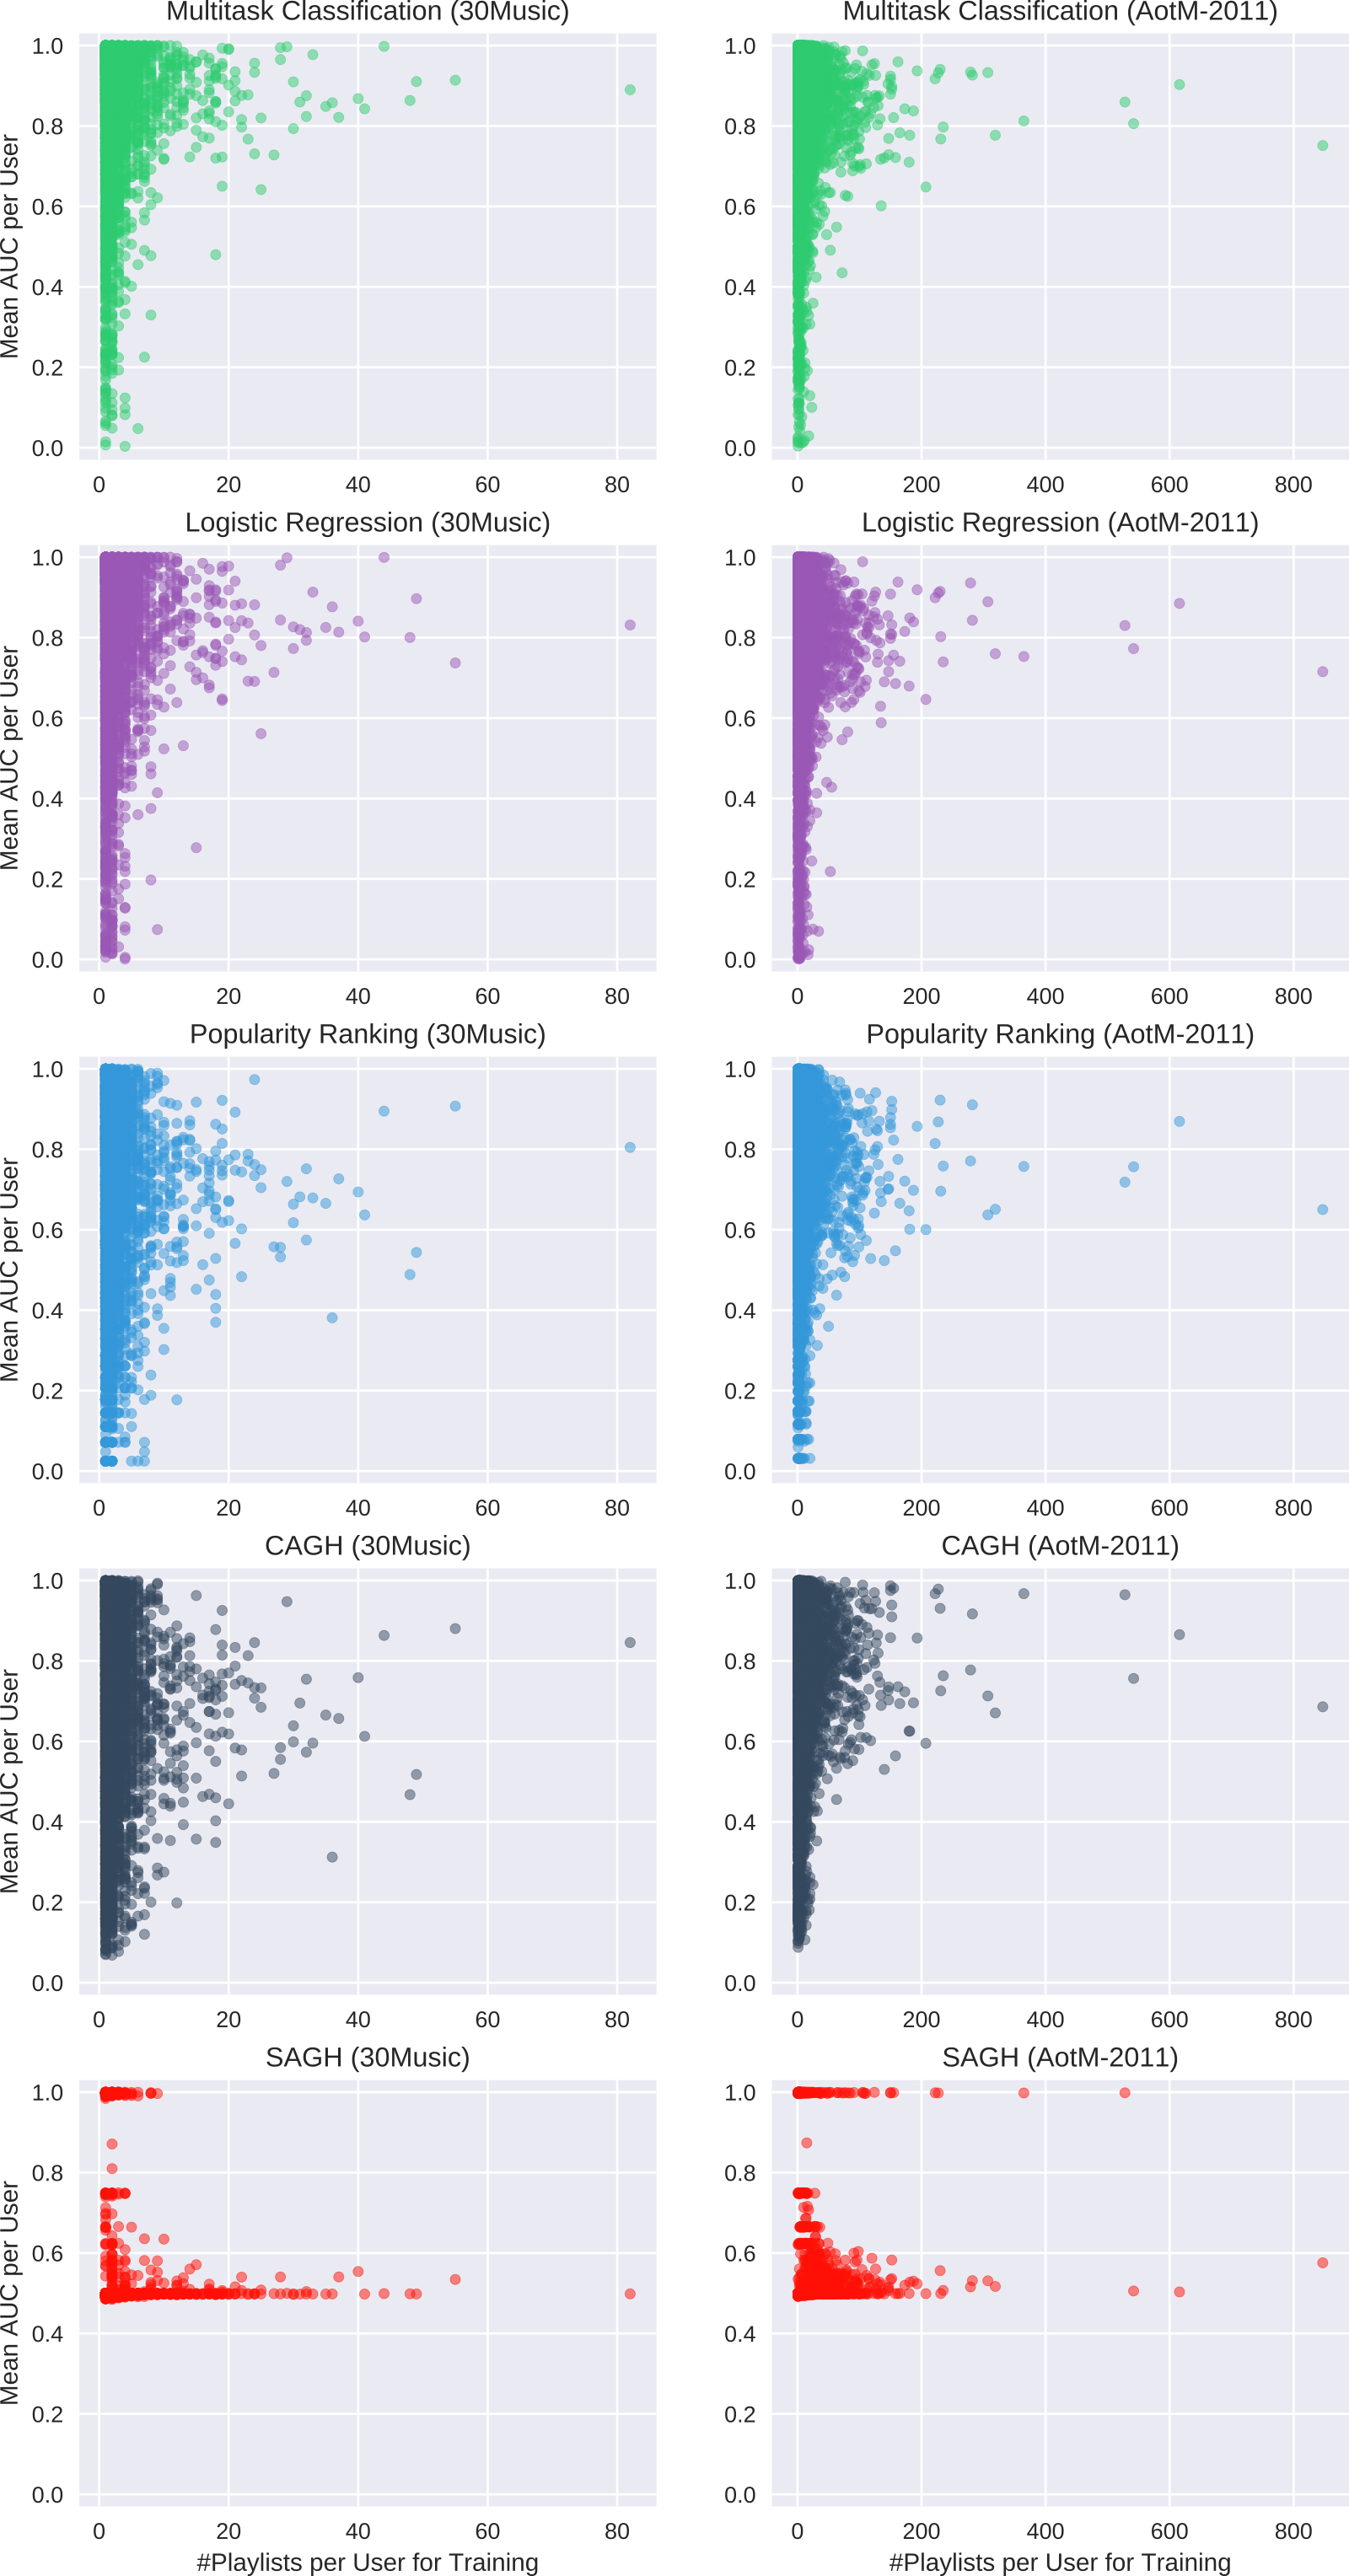
\includegraphics[height=\textheight]{fig/auc_per_user0.png}
    \caption{Performance (AUC) per User in \emph{Cold Songs} Setting}
    %\label{}
\end{figure}

\begin{figure}[!t]
    \centering
    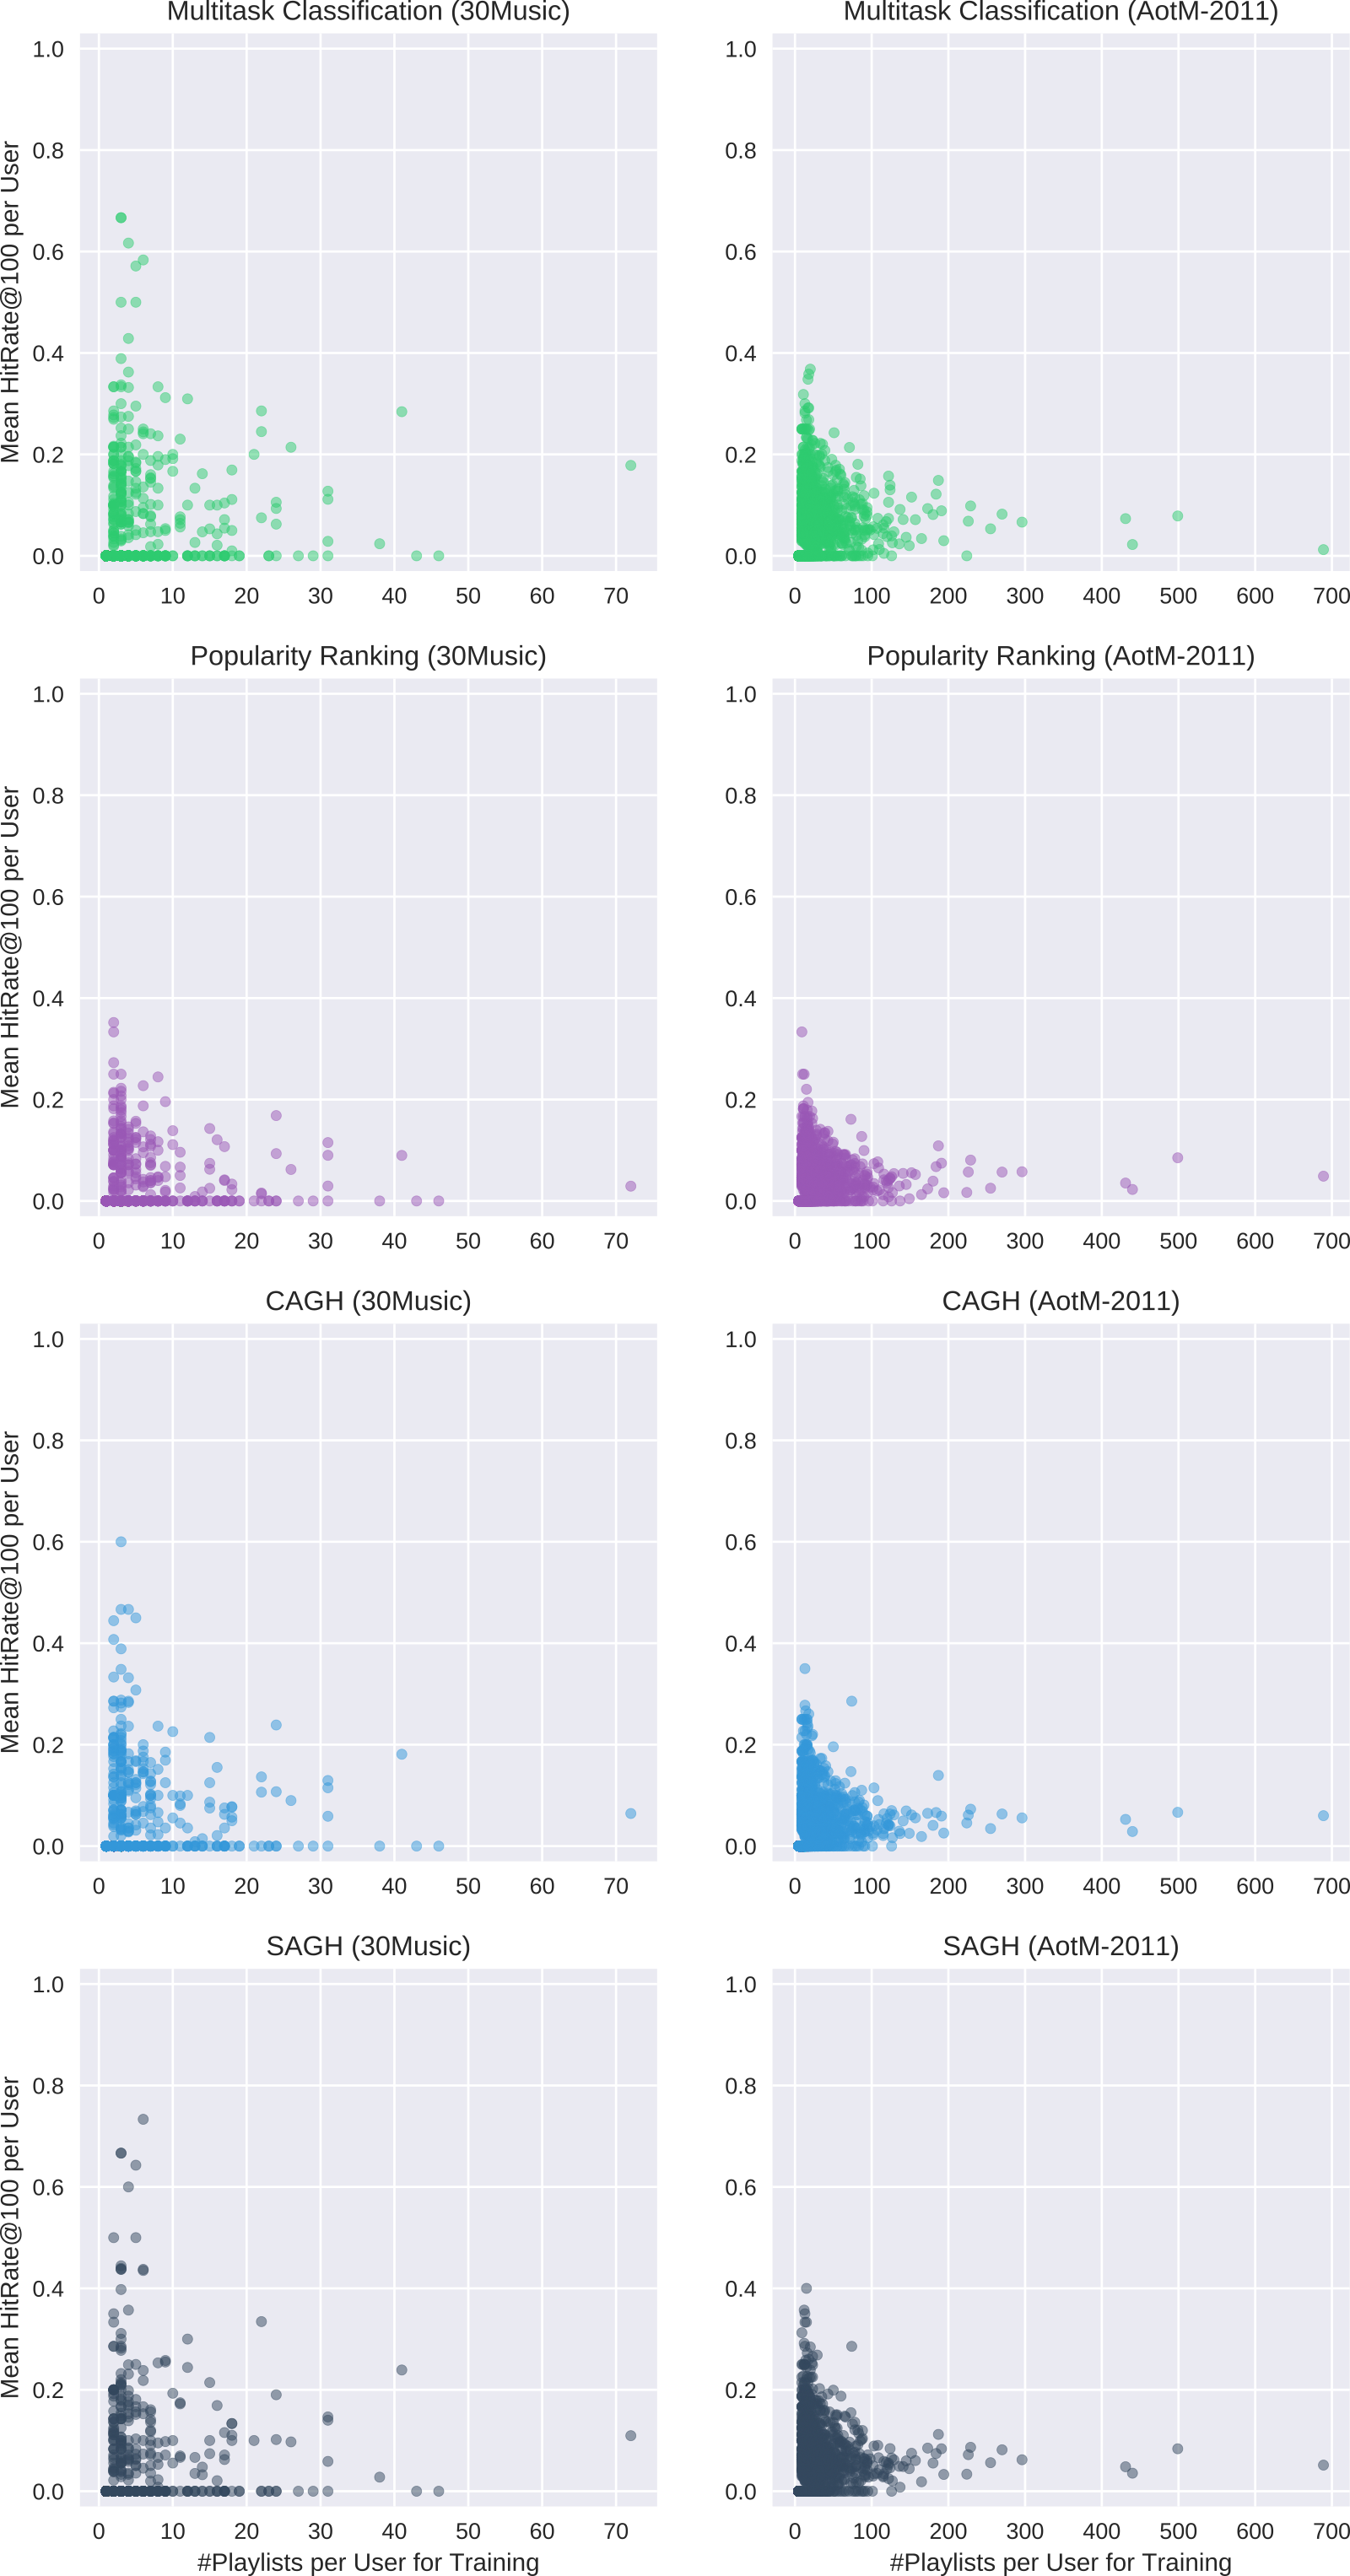
\includegraphics[height=\textheight]{fig/hitrate_per_user1.png}
    \caption{Performance (HitRate@100) per User in \emph{Cold Playlists} Setting}
    %\label{}
\end{figure}

\begin{figure}[!t]
    \centering
    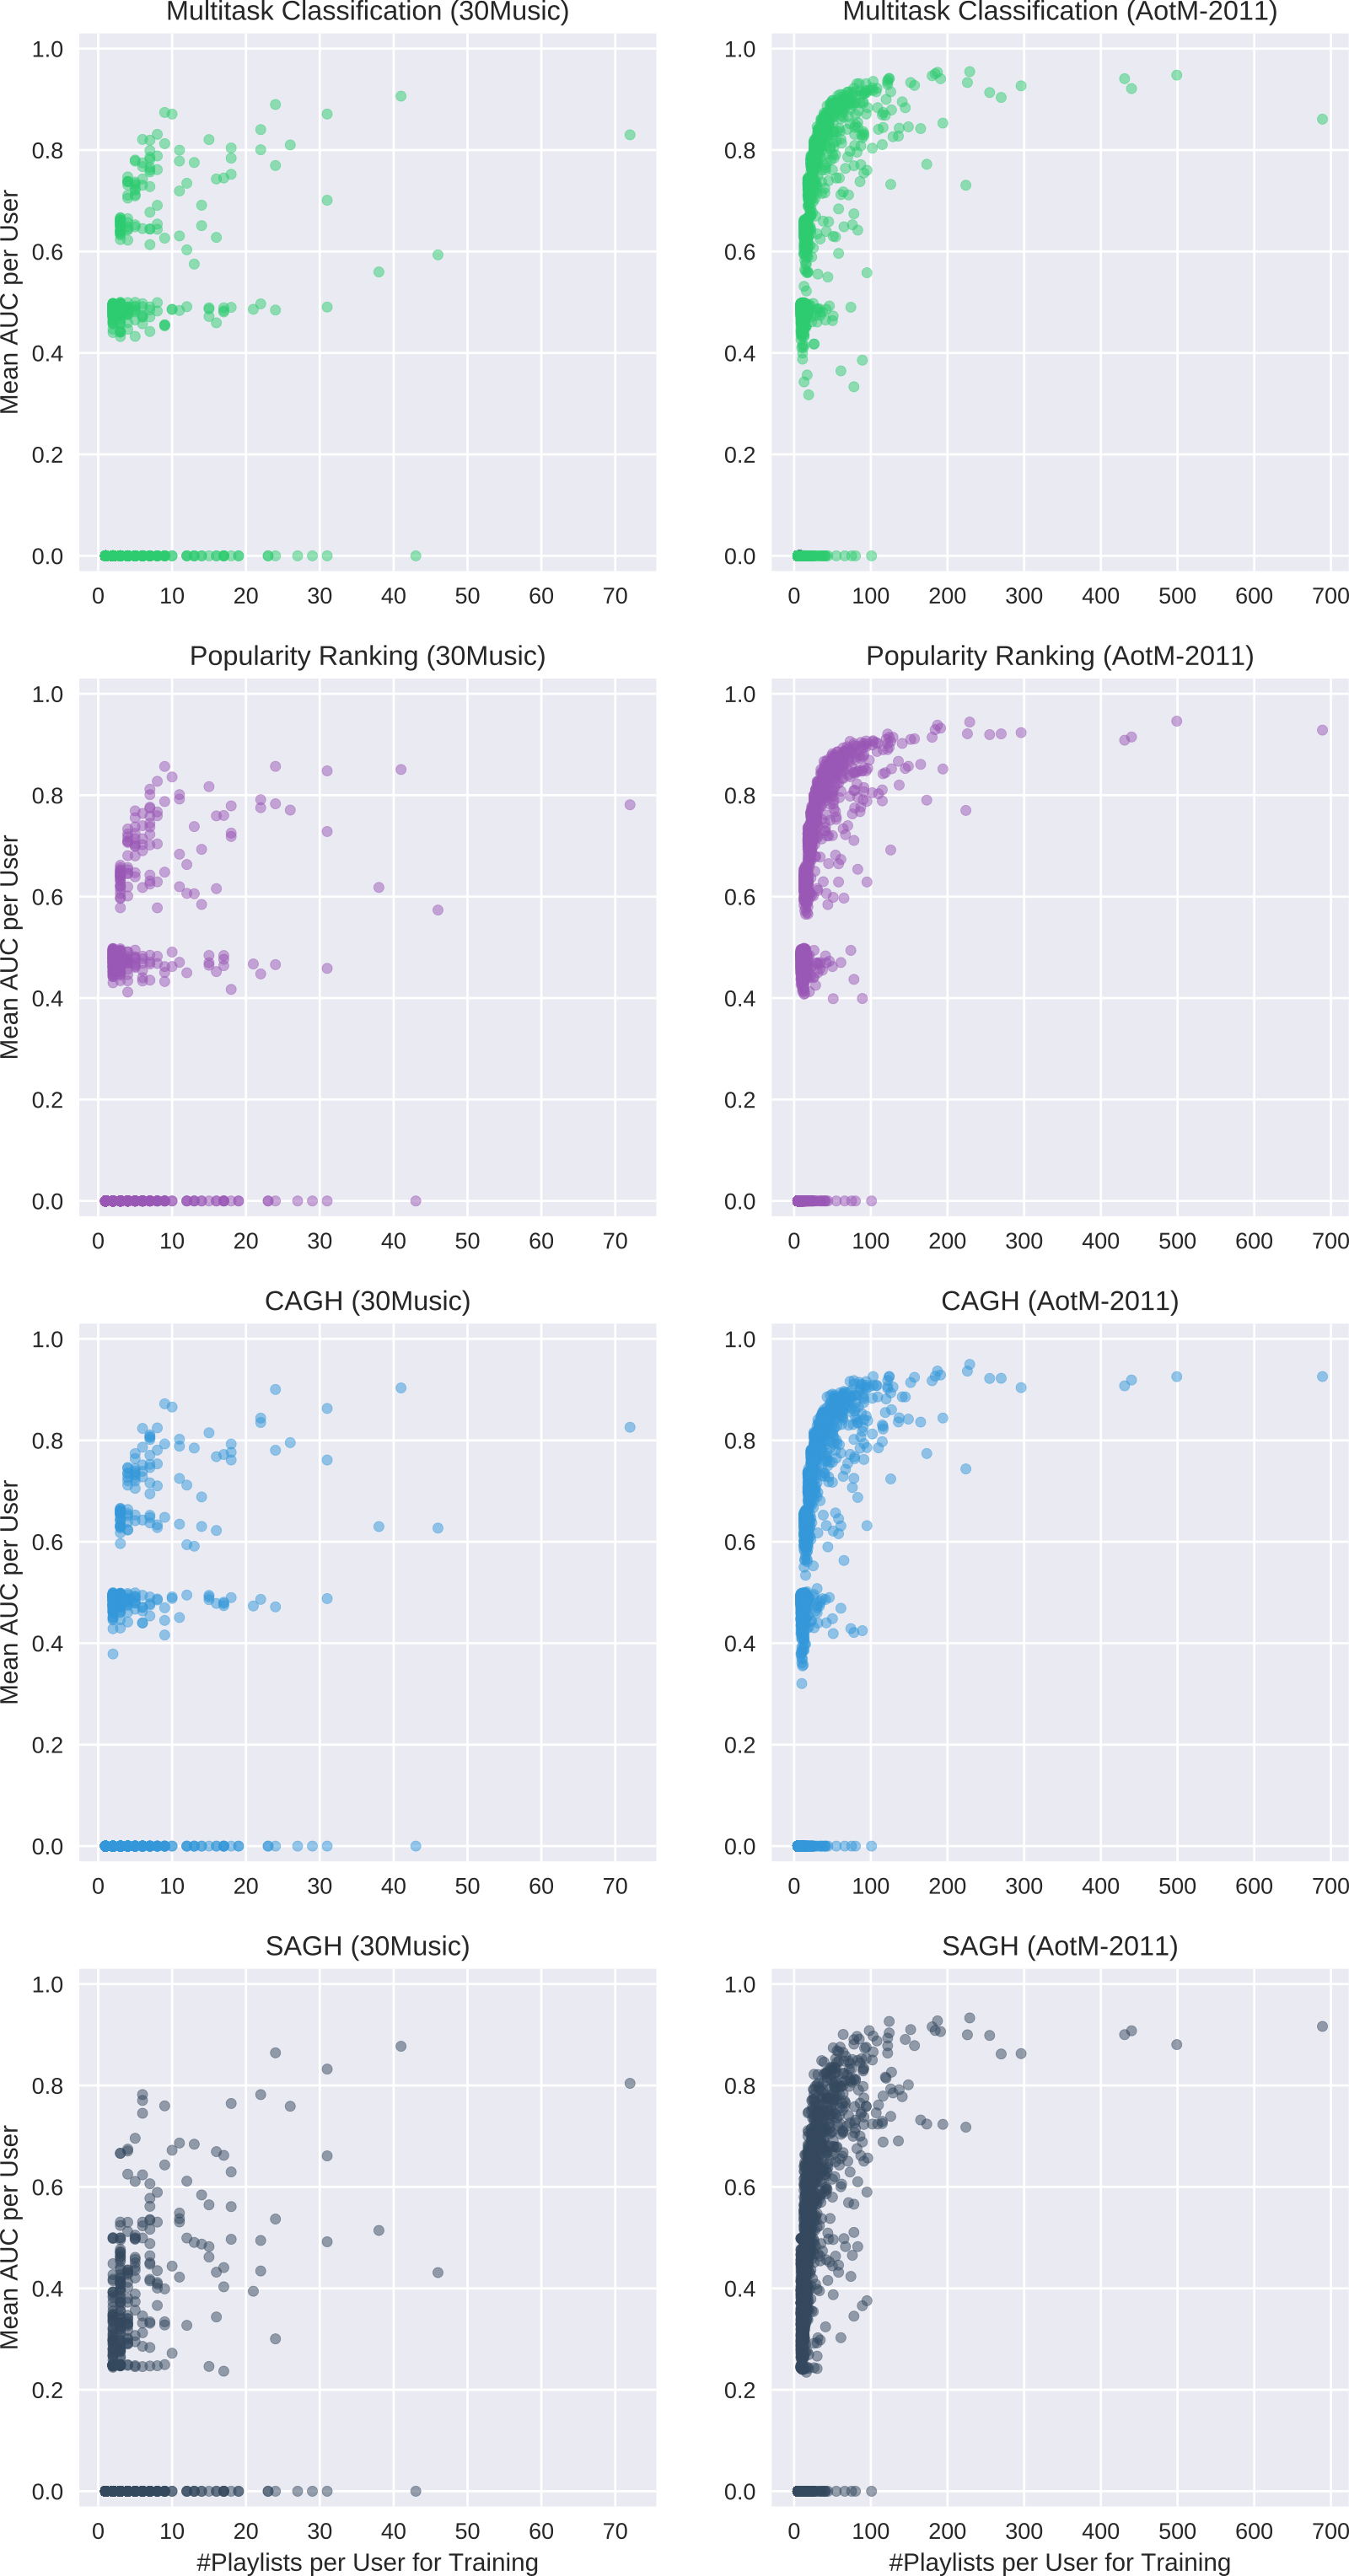
\includegraphics[height=\textheight]{fig/auc_per_user1.png}
    \caption{Performance (AUC) per User in \emph{Cold Playlists} Setting}
    %\label{}
\end{figure}


\begin{figure*}[!h]
    \centering
    \begin{minipage}{0.45\textwidth}
        \centering
        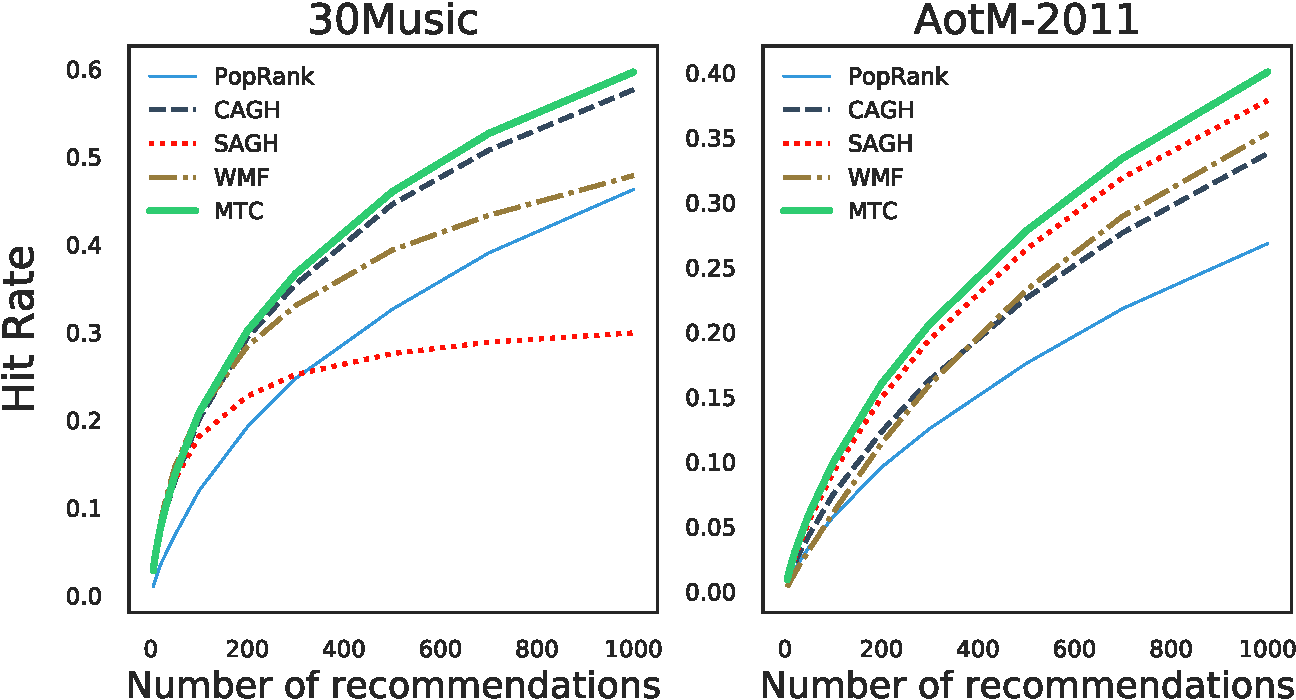
\includegraphics[width=\linewidth]{fig/hr3.pdf}
        \caption{Hit rate of recommendation in the \emph{cold playlists} setting. \emph{Higher} values indicate better performance.}
        \label{fig:hr3}
    \end{minipage}\hspace{15pt}
    \begin{minipage}{0.45\textwidth}
        \centering
        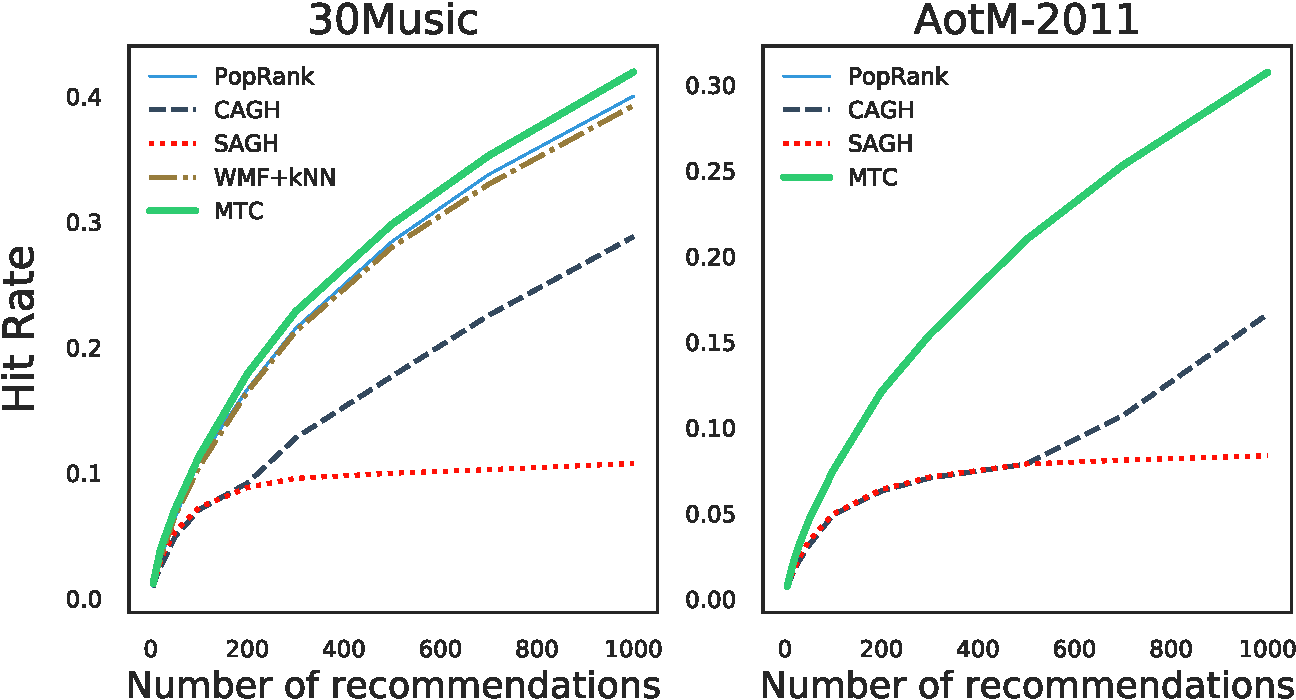
\includegraphics[width=\linewidth]{fig/hr4.pdf}
        \caption{Hit rate of recommendation in the \emph{cold users} setting. \emph{Higher} values indicate better performance.}
        \label{fig:hr4}
    \end{minipage}
\end{figure*}

\begin{figure*}[!h]
    \centering
    \begin{minipage}{0.45\textwidth}
        \centering
        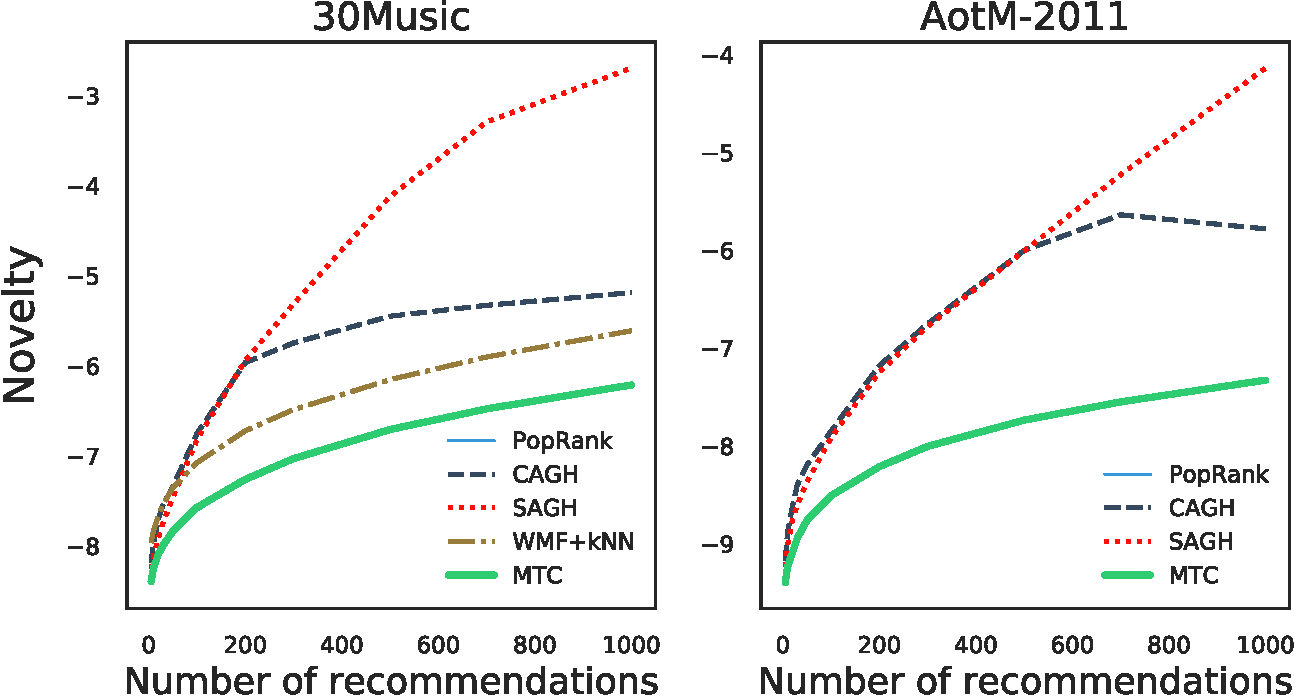
\includegraphics[width=\columnwidth]{fig/nov4.pdf}
        \caption{Novelty of recommendation in the \emph{cold users} setting. \emph{Moderate} values are preferable.}
        \label{fig:nov4}
    \end{minipage}\hspace{15pt}
    \begin{minipage}{0.45\textwidth}
        \centering
        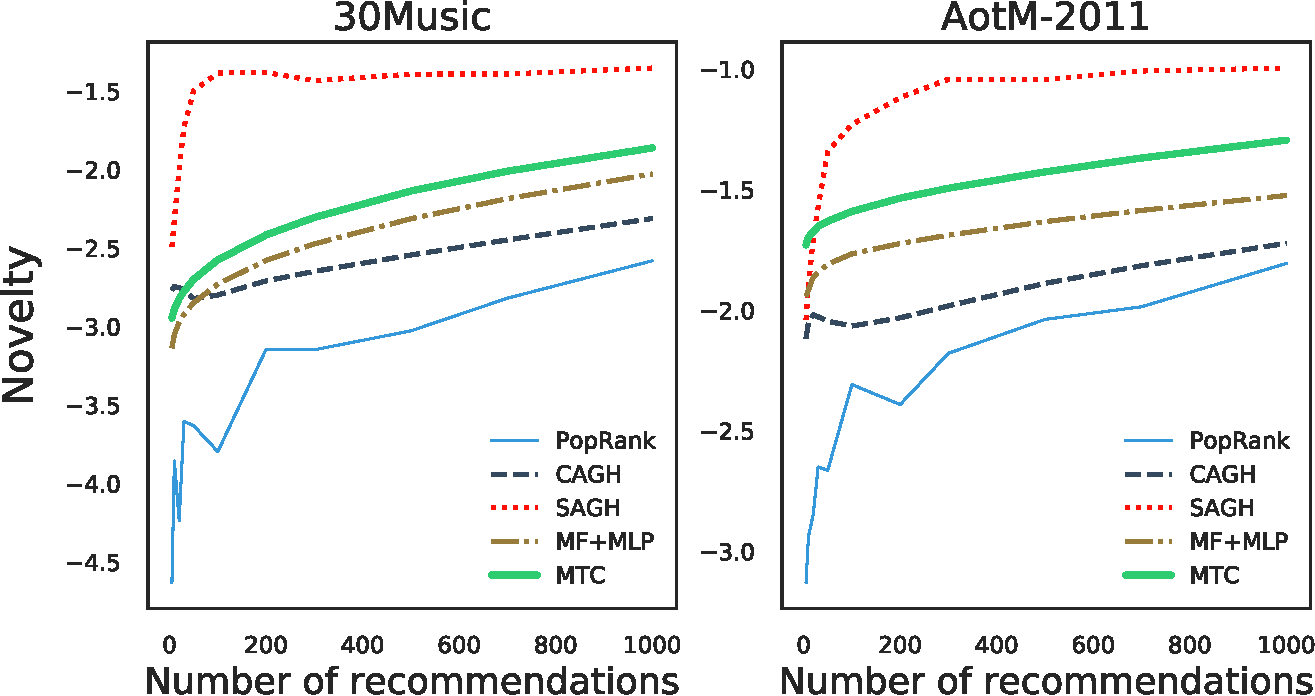
\includegraphics[width=\columnwidth]{fig/nov1.pdf}
        \caption{Novelty of recommendation in the \emph{cold songs} setting. \emph{Moderate} values are preferable.}
        \label{fig:nov1}
    \end{minipage}
\end{figure*}


\clearpage
\newpage
\onecolumn

%\section{Notations}
\section{Notations}

We introduce notations in Table~\ref{tab:symbol_tpush}.
\begin{table}[!h]
\caption{Glossary of commonly used symbols}
\label{tab:symbol_tpush}
\renewcommand{\arraystretch}{1.5} % tweak the space between rows
\setlength{\tabcolsep}{1pt} % tweak the space between columns
\centering
\begin{tabular}{llll}
\toprule
\multicolumn{3}{l}{\textbf{Notation}} & \textbf{Description} \\ \midrule
$D$        &  $\in$  &  $\Z^+$            & The number of features for each song \\
$M$        &  $\in$  &  $\Z^+$            & The number of songs, indexed by $m, n \in \{1,\dots,M\}$ \\
$N$        &  $\in$  &  $\Z^+$            & The number of playlists, indexed by $i \in \{1,\dots,N\}$ \\
$U$        &  $\in$  &  $\Z^+$            & The number of users, indexed by $j \in \{1,\dots,U\}$ \\
$\bv_i$    &  $\in$  &  $\R^D$            & The weights of playlist $i$ \\
$\bu_j$    &  $\in$  &  $\R^D$            & The weights of user $j$ \\
$\widebar\bu$    &  $\in$  &  $\R^D$      & The weights shared by all playlists \\
$\w_i    $ &  $\in$  &  $\R^D$            & The weights for playlist $i$ that owned by user $j=u(i)$, $\w_i = \bv_i + \bu_j + \widebar\bu$ \\
$\Y$       &  $\in$  &  $\R^{M \times N}$ & The matrix of binary labels that indicating if a song is in a playlist \\
$y_m^k$    &  $\in$  &  $\R^D$            & The positive binary label $y_m^k = 1$, \ie song $m$ in playlist $k$ \\
$y_n^k$    &  $\in$  &  $\R^D$            & The negative binary label $y_n^k = 0$, \ie song $n$ not in playlist $k$ \\
$\X$       &  $\in$  &  $\R^{M \times D}$ & The matrix of features of all songs \\
$\x_m$     &  $\in$  &  $\R^D$            & The feature vector of song $m$ \\
$\x_n$     &  $\in$  &  $\R^D$            & The feature vector of song $n$ \\
\bottomrule
\end{tabular}
\end{table}

